%
% Copyright (c) 2013-2023 Aleksey Fedoseev <aleksey@fedoseev.net>
% Copyright (c) 2013-2015 Nikolay Safronov <bfishh@gmail.com>
% 
% Permission is granted to copy, distribute and/or modify this document
% under the terms of the GNU Free Documentation License, Version 1.3
% or any later version published by the Free Software Foundation;
% with no Invariant Sections, no Front-Cover Texts, and no Back-Cover Texts.
% A copy of the license is located here: http://www.gnu.org/copyleft/fdl.html.
%

\documentclass[12pt,a4paper]{article}
\usepackage[T2A]{fontenc}
\usepackage{ucs}
\usepackage[utf8]{inputenc}
\usepackage[english,russian]{babel}
\usepackage{indentfirst}
\usepackage{amsmath}
\usepackage{amssymb}
\usepackage{graphicx}
\usepackage{hyperref}
\usepackage{array}
\usepackage{titlesec}
\usepackage{subcaption}
\usepackage{wasysym}
\usepackage{longtable}

\pagestyle{plain}
\parindent=1.25cm
\textheight=24cm
\textwidth=16cm
\topmargin=-1cm
\frenchspacing
\renewcommand{\theequation}{\thesection.\arabic{equation}}
\newcommand{\sectionbreak}{\clearpage}

\begin{document}

\title{%
  \textbf{Инженерный симулятор ОРБИТА 1.0} \\
    Руководство для преподавателя}

\author{
  Алексей Федосеев\\
  \texttt{aleksey@fedoseev.net}
  \and
  Николай Сафронов\\
  \texttt{bfishh@gmail.com}
}

\date{Версия 1.5, \today}

\maketitle

Этот текст распространяется под лицензией GNU Free Documentation License (FDL) версии
1.3. Подробную информацию об этой лицензии Вы можете на сайте GNU
\footnote{\url{http://www.gnu.org/copyleft/fdl.html}}.

Исходный текст находится в репозитории проекта на GitHub
\footnote{\url{https://github.com/dralex/orbita-simulator}}.

\tableofcontents

\clearpage
\section{Введение}

Мы предлагаем вам на время занять место Сергея Королева или Илона Маска и построить
собственную программу освоения Солнечной системы. Вы сможете конструировать свои
космические аппараты и отправлять их к ближайшим планетам~--- Луне, Марсу, Меркурию и
Венере. На каждой вас ждут новые испытания и невероятные открытия. Тем, кто сможет первым
посадить аппарат на планету или же доставить оттуда самую интересную научную информацию,
достанутся призы.

В вашем распоряжении конструктор космических аппаратов. В первых миссиях вы сможете
изменять один или несколько параметров корабля, а в последующих вам придется полностью
конструировать корабль из множества доступных компонентов.

Вам будут доступны результаты каждого полета~--- вы сможете узнать, что случилось с
кораблем, увидеть графики основных параметров полета, а также загрузить подробный журнал
телеметрии аппарата.

\section{Луна}

Луна~--- ближайший к Земле астрономический объект. Посадка корабля на Луну~--- это самое
простое задание, с которым человечество справлялось уже не раз. Это первая, тренировочная
задача, поэтому в ней есть много допущений: аппарат движется только вертикально, его
начальная скорость равна нулю, а из доступного оборудования на корабле есть только один
тормозной двигатель и демпфер.

\begin{figure}[tbh]
  \begin{center}
    \includegraphics[width=8cm]{images/moon1-ru.eps}
    \caption{Схема посадки аппарата на Луну}
    \label{Pic:moon1}
  \end{center}
\end{figure}

Задача состоит в том, чтобы определить, в какой момент времени $ t_1 $ нужно включить
тормозной двигатель, чтобы к моменту посадки $ t_2 $ скорость корабля была бы меньше \emph{50
м/с}, иначе удар не удастся самортизировать с помощью демпфера.

Другими словами, нужно вычислить один-единственный параметр~--- \emph{время включения
  тормозного двигателя}.

Все исходные данные известны: это начальная высота, масса и радиус Луны, масса аппарата,
сила тормозного двигателя.

\subsection{Исходные данные}

\begin{center}
\begin{tabular}{ |c|p{6cm}|p{6cm}| } 
  \hline
  \textbf{Параметр} & \textbf{Пояснение} & \textbf{Значение} \\
  \hline
  $ H $ & Высота схода аппарата с орбиты (начало падения) & \emph{50 000 м (50 км)} \\
  \hline
  $ G $ & Гравитационная постоянная & $ 6,6742 \cdot 10^{-11} \text{Н} \text{м}^{2}/\text{кг}^{2} $ \\
  \hline
  $ M $ & Масса Луны & $7,35 \cdot 10^{22} \text{кг}$ \\
  \hline
  $ R $ & Радиус Луны & \emph{1 737 100 м (1737 км)} \\
  \hline
  $ a_{\text{дв}} $ & Ускорение, сообщаемое аппарату тормозным двигателем & Вычисляется по формуле:
  $ a_{e} = F_{\text{дв}} / m $ (второй закон Ньютона), $ \text{м}/\text{с}^2 $ \\
  \hline  
  $ m $ & Масса аппарата & В начале полета масса равна \emph{2935,88 кг}, из них аппарат
  содержит $m_{\text{т}} = 500 $ \emph{кг} топлива.\\
  \hline
  $ F_{\text{дв}} $ & Сила тяги тормозного двигателя, используемого на данном аппарате &
  Вычисляется по формуле: $ F_{\text{дв}} = u \cdot \Delta m$.\\
  \hline
  $ u $ & Скорость истечения газов из сопла двигателя & \emph{3600 м/c}\\
  \hline
  $ \Delta m $ & Тяга (расход топлива) & \emph{4,2 кг/c}\\
  \hline
\end{tabular}
\end{center}

\subsection{Шаг первый: аналитическое решение}

Давайте попробуем решить эту задачу аналитически. Для этого сделаем два допущения:

\begin{enumerate}
\item что масса корабля остается постоянной (топливо не расходуется);
\item а сила тяжести также не изменяется с высотой (высота аппарата мала по сравнению с
  радиусом Луны).
\end{enumerate}

В этом случае легко записать систему уравнений и решить ее. Время включения двигателей
можно получить по формуле (само решение системы уравнений есть в разделе \ref{Sec:Moon-Model})

$$ t_1 = \sqrt{2 H \left(\frac{1}{g} - \frac{1}{a_{\text{дв}}}\right)} =
\sqrt{2 H \left(\frac{r^2}{G M} - \frac{m}{F_{\text{дв}}}\right)} $$,

где $r$ - высота аппарата, которая меняется в интервале от $(H + R)$ до $R$, а $m$~---
масса аппарата, которая на самом деле в ходе полета может уменьшиться до величины $(m -
m_{\text{т}})$ в результате расхода топлива.

\hfill

\noindent\fbox{\parbox{\textwidth}{%
    Возьмите какие-нибудь значения высоты и массы из указанных диапазонов и запустите аппарат
    с полученным временем включения двигателей.
}}

\subsection{Шаг второй: программа полета}

Для управления полетом в симуляторе можно использовать два режима:

\begin{description}
\item[таблица команд] содержит последовательность команд, представляющих собой изменение
  режима аппарата в заданные моменты времени;
\item[код программы на языке Python] содержит полноценную программу управления.
\end{description}  

Пример таблицы с командами для первой миссии, обратите внимание, что для каждой команды
указывается уникальный идентификатор устройства (например, \verb'EG1'), получаемый из кода
типа устройства (\verb'EG') и номера (\verb'1'):

\begin{center}
\begin{tabular}{ |c|c|c|c| } 
  \hline
  \textbf{Время, с} & \textbf{Устройство} & \textbf{Новое состояние} & \textbf{Аргумент} \\
  \hline
  0 & D1 & PERIOD & 10 \\
  \hline
  $t_1$ & EG1 & TURNON & - \\
  \hline
\end{tabular}
\end{center}

Пример программы полета с включением двигателя в момент времени $t_1$:

\begin{verbatim}
t1 = # ВПИШИТЕ ВЫЧИСЛЕННОЕ ЗНАЧЕНИЕ t1
engine = False
probe.set_device_period('D1', 60)
while probe.run():
    t = probe.cpu_get_flight_time()
    if not engine and t >= t1:
        probe.set_device_state('EG1', STATE_ON)
        engine = True
        continue
    if probe.navigation_has_landed():
        break
\end{verbatim}

Более подробно о программах полета на языке Python рассказывается в Приложении 2.

\subsection{Шаг третий: анализ телеметрии}

По итогам запуска симулятора (не зависимо от успешности полета) вам будут доступны записи
телеметрии аппарата. Помимо общих сведений об аппарате, вы увидите таблицу изменений
основных параметров аппарата с течением времени:

\begin{verbatim*}
...
Ti=00:04:00 H=009561.8 Vy=-0162.7 Ac=003.9 Ae=005.5
Ti=00:04:10 H=008130.7 Vy=-0123.8 Ac=003.9 Ae=005.5
...
\end{verbatim*}

Возможные параметры телеметрии представлены в таблице:

\begin{center}
\begin{tabular}{ |c|c|p{2.5cm}|p{6cm}| } 
  \hline
  \textbf{Название} & \textbf{Код} & \textbf{Единица измерения} & \textbf{Комментарий} \\
  \hline
  Время полета & \textbf{Ti} & час:мин:сек & Период телеметрии \emph{10 сек}\\
  \hline
  Высота над поверхностью & \textbf{H} & м & Начальная высота \emph{50 000 м}\\
  \hline
  Вертикальная скорость & \textbf{Vy} & м/c & Начальная скорость равна
  \emph{0}. Напоминаем, что ось $y$ направлена вверх\\
  \hline
  Суммарное ускорение & \textbf{Ac} & $\text{м}/\text{с}^{2}$ & Абсолютное значение ускорения\\
  \hline
  Ускорение от двигателей & \textbf{Ae} & $\text{м}/\text{с}^{2}$ & Абсолютное значение ускорения,
  создаваемого включенным двигателем\\
  \hline
\end{tabular}
\end{center}

Результаты телеметрии также могут быть представлены графически:

\begin{figure}[tbh]
  \begin{center}
    \includegraphics[width=16cm]{images/telemetry.eps}
    \caption{Представление результатов телеметрии аппарата}
    \label{Pic:telemetry}
  \end{center}
\end{figure}

\hfill

\noindent\fbox{\parbox{\textwidth}{%
    Используя данные телеметрии, постройте графики изменения скорости и высоты. Объясните
    качественное изменение этих величин.
}}

\subsection{Шаг четвертый: переход от аналитического решения к фактическому}

Аналитическое решение не дает точного правильного ответа: для некоторых значений $t_1$
аппарат разбивается. Это связано с тем, что изменениями массы и высоты аппарата нельзя
пренебречь:

$$ t_1 = \sqrt{2 H \left(\frac{r^2}{G M} - \frac{m}{F_{\text{дв}}}\right)} $$,

Из формулы видно, что в течение полета уменьшаются оба числителя. Можно оценить крайние
значения $t_1$, а также значение времени для средних величин $r$ и $m$. Правильный ответ будет
лежать в этой области.

\hfill

\noindent\fbox{\parbox{\textwidth}{%
    Используйте результат первого полета, чтобы понять,
    должны ли вы уменьшить или увеличить время включения тормозного
    двигателя. Ориентируйтесь на диапазон значений $t_1$, полученных из аналитического
    решения. Посадите корабль на Луну за минимальное число попыток.
}}

\subsection{Как было получено аналитическое решение}
\label{Sec:Moon-Model}

Разделим спуск аппарата на два промежутка времени: от начала движения до включения
тормозного двигателя $(0; t_1)$, и от включения двигателя до касания поверхности $(t_1;
t_2)$. Для первого этапа уравнение движения имеет вид:

$$
y_1 = H - \frac{g t^2_1}{2}
$$

Это падение под действием силы тяжести, где $g$ рассматривается как константа и равно $ g
= \frac{G M}{R^2}$.

Для второго этапа полета:

$$
y_2 = y_1 - v_{\text{дв}} t_2 + \frac{a t^2}{R^2},
$$

где $ v_{\text{дв}} = g t_1$~--- абсолютное значение, набранное в результате начального падения, а
$a = a_{\text{дв}} - g$ (общее ускорение, состоящее из ускорения свободного падения $g$ и
ускорения, сообщаемого двигателями $a_{\text{дв}}$).

Суммарно проделанный аппаратом путь равен высоте, с которой началось падение, поэтому:

$$
y_2 = 0
$$

Нам необходимо подобрать момент включения двигателя ($t_1$) так, чтобы скорость
($v_{\text{дв}}$), набранная за первый этап, была полностью погашена за время второго
этапа (движение с включенным двигателем до посадки), т.е:

$$
v_{\text{дв}} = a t_2
$$

Все эти соображения дают нам систему уравнений, решив которую, мы сможем найти оптимальное
время включения двигателя. Система уравнений \ref{Eq:moon1}-\ref{Eq:moon6}:

\begin{eqnarray}
  y_1 = H - \frac{g t^2_1}{2} \label{Eq:moon1} \\
  y_2 = y_1 - v_{\text{дв}} t_2 + \frac{a t^2}{R^2} \label{Eq:moon2}\\
  y_2 = 0 \label{Eq:moon3} \\
  v_{\text{дв}} = g t_1 \label{Eq:moon4} \\
  v_{\text{дв}} = a t_2 \label{Eq:moon5} \\
  a = a_{\text{дв}} - g \label{Eq:moon6}
\end{eqnarray}

Важно отметить следующие моменты:

\begin{enumerate}
\item ось $y$ направлена вверх, точка начала координат находится на поверхности планеты;
\item мы считаем, что $g$~--- константа (в реальности это не так);
\item мы пренебрегаем уменьшением массы аппарата, т.е. считаем что $a$~--- константа (в
  реальности это также неверно, ведь топливо на корабле вырабатывается).
\end{enumerate}  

Решение:

Выразим $t_2$ через $t_1$, используя уравнения \ref{Eq:moon4} и \ref{Eq:moon5}.

\begin{eqnarray}
  g t_1 = a t_2 \nonumber \\
  t_2 = \frac{g t_1}{a} \label{Eq:moon7}
\end{eqnarray}

Поставим в уравнение \ref{Eq:moon2} $y_1$ и $y_2$ из уравнений \ref{Eq:moon1} и
\ref{Eq:moon3}.

$$
\begin{array}{c}
  0 = H - \frac{g t^2_1}{2} - v_{\text{дв}}t_2 + \frac{a t^2}{R^2}\\
  \text{или} \frac{g t^2_1}{2} + v_{\text{дв}}t_2 - \frac{a t^2}{R^2} = H
\end{array}
$$

Заменим $v_{\text{дв}}$ на его значение из уравнения \ref{Eq:moon4}:

$$
\frac{g t_1^2}{2} + g t_1 t_2 - \frac{a t_2^2}{2} = H
$$

Подставим значение  $t_2$ из уравнения \ref{Eq:moon7}:

$$
\begin{array}{c}
  \frac{g t_1^2}{2} + g t_1 \frac{g t_1}{a} - \frac{a}{2} \left(\frac{g t_1^2}{a}\right) =
  H \Rightarrow \\
  \frac{g t_1^2}{2} + \frac{g^2 t_1^2}{a} - \frac{g^2 t_1^2}{2 a} = H \Rightarrow \\
  a g t_1^2 + 2 g^2 t_1^2 - g^2 t_1^2 = 2 a H \Rightarrow \\
  t_1^2 \left(ag + g^2\right) = 2aH \Rightarrow \\
  t_1 = \sqrt{\frac{2 a H}{\left(a g + g^2\right)}}
\end{array}
$$

Подставим значение $a$ из уравнения \ref{Eq:moon6}:

$$
\begin{array}{c}
  t_1 = \sqrt{\frac{2 \left(a_{\text{дв}} - g\right) H}{\left((a_{\text{дв}} - g) g + g^2\right)}} \Rightarrow \\
  t_1 = \sqrt{2 H \frac{\left(a_{\text{дв}} - g\right)}{a_{\text{дв}} g}} \Rightarrow \\
    t_1 = \sqrt{2 H \left(\frac{1}{g} - \frac{1}{a_{\text{дв}}}\right)}  
\end{array}
$$

\section{Марс}

\emph{Красная Планета}~--- намного более сложный объект для посадки космического аппарата,
чем Луна. Во-первых, Марс намного массивнее, а значит сила тяжести играет куда большую
роль. Во-вторых, на Марсе есть атмосфера, так что влияние сопротивления атмосферы на
движение корабля около поверхности будет значительным. В этой задаче также есть ряд
упрощений: движение двумерно, а поверхность Марса рассматривается как плоскость.

При посадке на Марс в вашем распоряжении снова будет полностью сконструированный аппарат,
но вам придется самостоятельно \textbf{запрограммировать} его полет: выбрать, в какой
момент нужно будет включить тормозной двигатель, открыть парашют и т.д.

\begin{figure}[tbh]
  \begin{center}
    \includegraphics[width=8cm]{images/mars1-ru.eps}
    \caption{Схема посадки аппарата на Марс}
    \label{Pic:mars}
  \end{center}
\end{figure}

По сравнению с Луной задача усложняется: теперь придется работать в двух измерениях (хоть
и в плоских координатах). У аппарата есть начальная горизонтальная (орбитальная)
скорость. К тому же, теперь на аппарат действует не только сила тяжести, но и сила
аэродинамического сопротивления (Стокса), пропорциональная квадрату его скорости. Все это
делает аналитическое решение очень сложным, поэтому мы предлагаем вам качественно
оценивать значения скоростей и сил, а также тщательно анализировать результаты неудачных
полетов.

\subsection{Исходные данные}

\begin{center}
\begin{tabular}{ |c|p{6.5cm}|p{6cm}| } 
  \hline
  \textbf{Параметр} & \textbf{Пояснение} & \textbf{Значение} \\
  \hline
  $ G $ & Гравитационная постоянная & $ 6,6742 \cdot 10^{-11} \text{Н} \text{м}^{2}/\text{кг}^{2} $ \\
  \hline
  $ M $ & Масса Марса & $6,4185 \cdot 10^{23} \text{кг}$ \\
  \hline
  $ R $ & Радиус Марса & \emph{3 389 500 м (3389,5 км)} \\
  \hline
  $ H $ & Высота стартовой орбиты & \emph{80 000 м} \\
  \hline
  $ k $ & Аэродинамический коэффициент. Известен для сферического аппарата & 0,47 \\
  \hline
  $ S $ & Характерная площадь тела (площадь сечения аппарата, увеличивается на площадь
  теплового щита или парашюта, если он раскрыт) & вычисляется по формуле $ S = \pi r $, где $r$~--- радиус
  аппарата \\
  \hline
  $ r $ & Радиус аппарата & \emph{0,811 м} \\
  \hline
  $ m $ & Масса аппарата (на начало полета) & \emph{1397,61 кг} \\
  \hline
  $ v $ & Стартовая скорость аппарата (горизонтальная) & \emph{3555,07 м/с} \\
  \hline
  $ F_{\text{дв}} $ & Сила посадочного двигателя &
  Вычисляется по формуле: $ F_{\text{дв}} = u \cdot \Delta m$.\\
  \hline
  $ u $ & Скорость истечения газов из сопла двигателя & \emph{3600 м/c}\\
  \hline
  $ \Delta m $ & Тяга (расход топлива) & \emph{4,2 кг/c}, аппарат снабжен \emph{50 кг}
  топлива\\
  \hline
  $ V_{\text{демпф}}$ & Предельная скорость для амортизации демпфером & \emph{40 м/с} \\
  \hline
\end{tabular}
\end{center}

Аппарат оснащен следующими основными устройствами:

\begin{center}
\begin{tabular}{ |p{5cm}|c|p{8.5cm}| } 
  \hline
  \textbf{Название} & \textbf{Код} & \textbf{Назначение} \\
  \hline
  Аэродинамический тормоз (Тепловой щит) & \textbf{Hsl1} & Применяется при входе в
  атмосферу. Этот массивный щит используется для гашения основной скорости аппарата. \\
  \hline
  Парашют для разреженной атмосферы & \textbf{Pam1} & Огромный по площади парашют
  позволяет замедлить аппарат даже в разреженной атмосфере.\\ 
  \hline
  Посадочный двигатель & \textbf{EG1} & Двигатель с небольшой тягой, позволяющий
  скорректировать скорость посадки аппарата. \\
  \hline
  Демпфер & \textbf{Dm1} & Демпфер позволяет амортизировать лишнюю скорость при достижении
  поверхности. Здесь рассматривается упрощенная версия работы с демпфером на основе
  предельной скорости, более точный расчет можно
    произвести в опоре на поглощение кинетической энергии демпфером, о чем говорится в
    описании следующей миссии\\
  \hline
\end{tabular}
\end{center}

Каждое устройство можно \textbf{включить} или \textbf{выключить} (с помощью команд
<<TURNON>> и <<TURNOFF>> или соответствующих вызовов в прогремме на Python), указав
соответственно время включения или выключения в секундах от начала посадки.

Учтите, что:

\begin{itemize}
  \item парашют имеет ограничение по максимальной скорости~--- если парашют открыть
    слишком рано, его просто сорвет (см. таблицу далее);
  \item при отключении парашюта или аэродинамического тормоза они отбрасываются, а значит,
    их масса (см. таблицу далее) вычитается из массы аппарата, также не получится включить
    эти устройства несколько раз;
  \item \emph{нельзя} открывать парашют до того, как был отброшен аэродинамический тормоз~--- они
    запутаются, и их оба сорвет;
  \item паращют или аэродинамический тормоз \emph{можно} использовать вместе с двигателем;
  \item посадочный двигатель расходует топливо, аппарат снабжен топливным баком на
    \emph{50 кг} топлива;
  \item при посадке аппарата, двигатель отключается автоматически.
\end{itemize}

Еще одно ограничение, которое появляется на Марсе в связи с посадкой в атмосфере -
предельная перегрузка аппарата. Если ускорение аппарата превысит \emph{155
  $\text{м}/\text{с}^2$}, он будет разрушен перегрузкой.

Параметры парашюта и аэродинамического тормоза:

\begin{center}
\begin{tabular}{ |p{5cm}|c|c|c|p{3cm}| } 
  \hline
  \textbf{Название} & \textbf{Код} & \textbf{Площадь, $\text{м}^2$} & \textbf{Масса, кг} &
  \textbf{Предельная скорость, м/с} \\
  \hline
  Аэродинамический тормоз & \textbf{Hsl} & 18 & 150 & 7000 \\
  \hline
  Парашют для разреженной атмосферы & \textbf{Pam} & 200 & 10 & 600 \\
  \hline
\end{tabular}
\end{center}

Ограничения физической модели, которая используется при посадке на Марс, вы можете
посмотреть в приложении \ref{Sec:Mars-Model}.

\subsection{Шаг первый. Разбираемся c расчетами гравитационной модели}

Для посадки на Марс нам придется много использовать программу для расчетов на
Земле. Программа для расчетов позволяет получить траекторию свободного падения тела с
заданными параметрами на поверхность Марса (с учетом используемой физической модели
гравитации, атмосферы и т.п.).

Конструкция аппарата фиксирована, поэтому начнем с известных параметров:

\begin{itemize}
  \item характерная площадь тела: \emph{2,0663 $\text{м}^2$};
  \item масса: \emph{1397,61 кг};
  \item стартовое положение ($x$): \emph{0 м};
  \item стартовая высота ($y$): \emph{80 000 м};
  \item стартовая горизонтальная скорость ($V_x$): \emph{3555,0733 м/с};
  \item стартовая вертикальная скорость ($V_y$): \emph{0 м/с}.
\end{itemize}

\hfill

\noindent\fbox{\parbox{\textwidth}{%
Введите известные начальные значения в программу и определите скорость аппарата в момент
касания поверхности. Будет ли данная скорость скомпенсирована демпфером?
}}

\hfill

Вывод гравитационной модели представляет приблизительно следующий массив данных:

\begin{verbatim}
Ti=00 X=0000000.0 H=080000.0 Vx=3555.1 Vy=00000.0 Ang=00.0 Ac=003.6 As=000.2
Ti=10 X=0035896.5 H=079816.7 Vx=3553.2 Vy=-0035.9 Ang=00.6 Ac=003.6 As=000.2
Ti=20 X=0071063.2 H=079284.8 Vx=3551.2 Vy=-0071.2 Ang=01.1 Ac=003.6 As=000.2
...
\end{verbatim}

Параметры вывода повтарают уже знакомый нам журнал полета аппарата на Луне. Помимо
координат и компонент скорости в журнале представлен угол относительно стартового
горизонтального полета (\textbf{Ang}), абсолютные значения суммарного ускорения аппарата
(\textbf{Ac}) и ускорения аппарата, связанного с силой аэродинамического сопротивления
(\textbf{As}). Примеры графиков гравитационной модели представлены на рисунке:

\begin{figure}[tbh]
  \begin{center}
    \includegraphics[width=16cm]{images/gravitymodel.eps}
    \caption{Представление результатов гравитационной модели}
    \label{Pic:gravitymodel}
  \end{center}
\end{figure}

Свободное падения корабля приводит к катастрофе. Что же делать?

Посмотрим на доступное оборудование~--- на самом деле, с момента старта у включен тепловой
щит (\textbf{Hsl1}). Наш расчет этого не учитывал, ведь тепловой щит увеличивает эффективную
площадь на \textbf{18 $\text{м}^2$}.

\hfill

\noindent\fbox{\parbox{\textwidth}{%
Посчитайте новую характерную площадь тела как сумму площади аппарата и площади теплового
щита. Как изменилась вычисляемая скорость посадки? Достаточно
ли только теплового щита и демпфера для успешной посадки?
}}

\subsection{Шаг второй. Что использовать - двигатель или парашют?}

Чтобы еще как-то замедлить спуск, нужно посмотреть на оборудование корабля. Из подходящего
оборудования у нас есть двигатели и парашют.

Двигатели характеризуются скоростью реактивной струи (в данном случае \emph{3600 м/с}) и
мощностью, которая пропорциональна расходу топлива (в нашем случае \emph{4.2 кг/с}). Проведем
грубую оценку нашей возможности замедлить падение двигателями.

Используем формулу Циолковского для скорости ракеты:

$$
v = u \ln\left(\frac{M_1}{M_2}\right)
$$

где $u$~--- удельная тяга (скорость истечения струи), $M_1$~--- масса аппарата с топливом,
$M_2$~--- масса аппарата без топлива.

Подставим наши значения ($M_2$ получим путем вычитания массы топлива из общей массы) и
получим скорость, которую мы будем вырабатывать двигателем.

\hfill

\noindent\fbox{\parbox{\textwidth}{%
Сможет ли вычисленная по формуле скорость, получаемая за счет двигателей, скомпенсировать
разгон аппарата силой тяжести? (В реальности пользы от двигателя будет еще меньше, так
есть сопротивление среды и другие факторы).
}}

\hfill

Если двигатели позволяют скомпенсировать скорость падения (которую мы вычислили на
предыдущем шаге), надо использовать их при посадке. Иначе — использовать парашют для
дальнейшего снижения скорости.

\subsection{Шаг третий. Посадка с парашютом}

Как видно из конструкции корабля, на нем установлен Парашют для разряженной атмосферы
(\textbf{Pam1}). Нам важны следующие его характеристики: площадь (\emph{200 $\text{м}^2$})
и максимальная допустимая скорость (\emph{600 м/с}).

Как работать с площадью~--- понятно. Это величина, которая прибавляется к характерной
площади тела и влияет на силу аэродинамического сопротивления нашего аппарата.

Максимальная допустимая скорость~--- это та скорость которую выдерживает парашют. Если
скорость потока воздуха (она же скорость нашего аппарата) будет больше, то парашют сорвет.

Итак, когда же раскрывать парашют? С одной стороны, чем раньше~--- тем лучше, тем больше
времени он будет нас тормозить и тем сильнее снизится скорость. С другой стороны, если
открыть его на слишком большой скорости, его сорвет потоком.

Посмотрим на нашу программу расчетов. Скорость аппарата складывается из скоростей $V_x$ и
$V_y$. Результирующую скорость $V$ найдем по теореме Пифагора.

\hfill

\noindent\fbox{\parbox{\textwidth}{%
Используйте программу для расчетов, чтобы вычислить, на какой минуте будет достигнута
приемлемая для выпуска парашюта скорость?
}}

\hfill

Так мы получим момент времени, в который можно сбрасывать тепловой щит и, одновременно,
выпускать паращют.

\hfill

\noindent\fbox{\parbox{\textwidth}{%
Снова используйте программу для расчетов. Но в этот раз рассчитайте последний участок
траектории~--- спуск на парашюте. В качестве начальных условий (скорость, высота) нужно
взять результат из предыдущего запуска для того момента времени, когда мы выпускаем
парашют. С какой теперь скорость будет происходить касание поверхности планеты?
}}

\hfill

Не забывайте, что парашют и тепловой щит не могут быть активны одновременно, а также то,
что масса аппарата уменьшится на массу отброшенного щита.

\hfill

\noindent\fbox{\parbox{\textwidth}{%
Если скорости в момент касания не достаточно для компенсации демпфером, можно ли ее
компенсировать двигателями? Для этой оценки у нас есть предельная скорость, полученная на
предыдущем этапе.
}}

\subsection{Шаг четвертый. Финальное торможение}

Теперь нам предстоит решить вопрос, когда включать (и выключать) двигатели.

Если мы включим их слишком рано, корабль остановится на большой высоте, а потом когда
кончится топливо упадет и разобьется. Если включим поздно, то двигатели не успеют
затормозить корабль.

Точно математически решить эту задачу чрезвычайно сложно, так как движение нашего аппарата
с учетом всех действующих на него сил описывается сложным дифференциальным уравнением. Но
можно провести некоторые оценки. Для этого снова воспользуемся формулой Циолковского для
реактивного движения.

Поскольку мы знаем, какую скорость нам надо погасить (это та скорость на которой мы
столкнемся с поверхностью если не включим двигатель), то мы можем посчитать массу топлива
которую нам нужно для этого потратить.

$$
\begin{array}{c}

  v = u \ln\left(\frac{M_1}{M_2}\right) \\
  \frac{v}{u} = \ln\left(\frac{M_1}{M_2}\right) \\
  e^{\frac{v}{u}} = \frac{M_1}{M_2}
\end{array}
$$

\hfill

\noindent\fbox{\parbox{\textwidth}{%
Используя формулу Циолковского, оцените, в какой момент нужно включить тормозной
двигатель. Теперь можно конструировать корабль и отправляться к Марсу.
}}

\subsection{Физическая модель}
\label{Sec:Mars-Model}

Аппарат приближается к Марсу на известной высоте (80 км над поверхностью планеты) с
известной скоростью~--- первой космической, которая в свою очередь определяется по следующей
формуле:

$$
v = \sqrt{\frac{G \cdot M}{R}},
$$

где $G$~--- гравитационная постоянная, $M$ и $R$~--- масса и радиус Марса.

В целях упрощения мы рассматриваем только двумерную задачу с переходом от окружности к
плоской поверхности, так что скорость раскладывается на две перпендикулярные компоненты. В
начале вертикальная компонента скорости ($Vy$) равна нулю.

Далее изменение параметров корабля определяется следующим дифференциальным уравнением:

$$
\frac{dv}{dt} = \frac{G M}{(R + y)^2} - \frac{k \rho(y) v^2 S}{2 m} - \frac{F_{\text{дв}}}{m}
$$

где $v$~--— скорость аппарата, $y$~--— высота над поверхностью Марса, $\rho(y)$~--—
плотность атмосферы Марса в зависимости от высоты (экспоненциальная зависимость), k~--—
аэродинамический коэффициент (аппарат имеет сферическую форму, он известен), $S$~--— площадь
сечения аппарата, $m$~--— масса аппарата, $F_{\text{дв}}$ — сила тормозных двигателей.

Видно, что в общем случае на аппарат воздействуют только три силы (гравитационная,
аэродинамического сопротивления по Стоксу и двигателей). На самом деле, так выглядит
формула для вертикального движения. При движении по горизонтали компонента силы тяжести
будет равна нулю. Данное уравнение приведено для скалярных величин, причем
аэродинамическое сопротивление направлено всегда против вектора скорости, а сила
двигателей~--- против силы тяжести.

График плотности атмосферы Марса, используемый в модели, представлен на рисунке
\ref{Pic:mars_atmosphere}.

\begin{figure}[tbh]
  \begin{center}
    \includegraphics[width=10cm]{images/mars-atm.eps}
    \caption{График изменения плотности атмосферы Марса}
    \label{Pic:mars_atmosphere}
  \end{center}
\end{figure}

Плотность атмосферы Марса меняется от \textbf{0,026 $\text{кг}/\text{м}^3$} на поверхности
до приблизительно нуля на высоте \textbf{80 000 м}, откуда аппарат начинает снижение.

\subsection{Анализ телеметрии}

Вам доступны записи телеметрии аппарата для всех совершенных полетов. Помимо общих
сведений об аппарате, вы увидите таблицу изменений основных параметров аппарата с течением
времени:

\begin{verbatim*}
Ti=00:03:17 X=0616595.0 H=016504.3 Vx=2371.1 Vy=-0590.0
 Ac=13.74 Ae=000.0 As=016.2
...
\end{verbatim*}

Возможные параметры телеметрии представлены в таблице:

\begin{center}
\begin{tabular}{ |c|c|p{2.5cm}|p{6cm}| } 
  \hline
  \textbf{Название} & \textbf{Код} & \textbf{Единица измерения} & \textbf{Комментарий} \\
  \hline
  Время полета & \textbf{Ti} & час:мин:сек & Период телеметрии \emph{1 сек}\\
  \hline
  Горизонтальное положение & \textbf{X} & м & Начальное положение берется за \emph{0}\\
  \hline
  Высота над поверхностью & \textbf{H} & м & Начальная высота \emph{50 000 м}\\
  \hline
  Горизонтальная скорость & \textbf{Vx} & м/c & Начальная скорость равна первой
  космической для Марса\\
  \hline
  Вертикальная скорость & \textbf{Vy} & м/c & Начальная скорость равна
  \emph{0}. Напоминаем, что ось $y$ направлена вверх\\
  \hline
  Угол ориентации аппарата & \textbf{Ang} & ° & Угол аппарата относительно начального положения (0°-90°)\\
  \hline
  Суммарное ускорение & \textbf{Ac} & $\text{м}/\text{с}^{2}$ & Абсолютное значение ускорения\\
  \hline
  Ускорение от двигателей & \textbf{Ae} & $\text{м}/\text{с}^{2}$ & Абсолютное значение ускорения,
  создаваемого включенным двигателем\\
  \hline
  Ускорение силы Стокса & \textbf{As} & $\text{м}/\text{с}^{2}$ & Абсолютное значение ускорения,
  создаваемого силой аэродинамического сопротивления\\
  \hline
\end{tabular}
\end{center}

\section{Меркурий}

Меркурий~--- одна из загадочных планет солнечной системы. При, казалось бы, небольшой
удаленности от Земли, эта планета до сих пор исследована довольно слабо. Тем интереснее
вызов~~--- разработать и посадить на Меркурий собственную автоматическую станцию.

Посадка на Меркурий напоминает посадку на Луну: отсутствие атмосферы, то же вертикальное
движение. Однако, на этот раз вам предстоит самостоятельно полностью разработать
конструкцию аппарата и его программу полета.

\begin{figure}[tbh]
  \begin{center}
    \includegraphics[width=8cm]{images/mercury-ru.eps}
    \caption{Схема посадки аппарата на Меркурий}
    \label{Pic:mercury}
  \end{center}
\end{figure}

Аппарат, достигший поверхности, начнет передавать на Землю научные результаты. Победителем
станет тот, кто не просто посадит аппарат на поверхность Меркурия первым, но сможет
оборудовать аппарат максимальным числом работающих научных приборов.

\subsection{Исходные данные}

\begin{center}
\begin{tabular}{ |c|p{6.5cm}|p{6cm}| } 
  \hline
  \textbf{Параметр} & \textbf{Пояснение} & \textbf{Значение} \\
  \hline
  $ G $ & Гравитационная постоянная & $ 6,6742 \cdot 10^{-11} \text{Н} \text{м}^{2}/\text{кг}^{2} $ \\
  \hline
  $ M $ & Масса Меркурия & $3,33 \cdot 10^{23} \text{кг}$ \\
  \hline
  $ R $ & Радиус Меркурия & \emph{2 439 700 м (2439,7 км)} \\
  \hline
  $ \rho_c $ & Плотность конструкции аппарата & \emph{100 $\text{кг}/\text{м}^3$} \\
  \hline
  $ F_{\text{дв}} $ & Сила посадочного двигателя &
  Вычисляется по формуле: $ F_{\text{дв}} = u \cdot \Delta m$, в которой скорость выброса
  и расход топлива зависят от используемого двигателя.\\
  \hline
\end{tabular}
\end{center}

Вам не придется конструировать аппарат с нуля. В вашем распоряжении будет сферический
аппарат, размер которого вы можете установить самостоятельно. Все, что вам нужно сделать -
выбрать необходимое для посадки оборудование и научные приборы так, чтобы их общий объем и
допустимая масса аппарата не превысили допустимых значений. Также вам придется следить за
уровнем энергоснабжения в корабле, чтобы всем системам хватало энергии. Помимо конструкции
аппарата, вам предстоит разработать и программу полета, например, определить время, когда
должны включаться и выключаться тормозные двигатели. При создании аппарата необходимо
учитывать предельные ограничения по массе (\textbf{20 тонн}) и радиусу внешней сферы
(\textbf{2 м}).

\begin{figure}[tbh]
  \begin{center}
    \includegraphics[width=10cm]{images/mercury-probe-ru.eps}
    \caption{Конструкция аппарата на Меркурии}
    \label{Pic:mercury-probe}
  \end{center}
\end{figure}

При посадке на Меркурий могут использоваться следующие двигатели и топливные баки:

\begin{center}
\begin{tabular}{ |p{2.5cm}|c|p{1.5cm}|p{1.5cm}|p{2cm}|p{2cm}|p{2.5cm}| } 
  \hline
  \textbf{Название} & \textbf{Код} & \textbf{Масса, кг} & \textbf{Объем, $\text{м}^3$} &
  \textbf{Скорость, м/с} & \textbf{Потр. энергии, * 10 Вт} & \textbf{Параметр}\\
  \hline
  Двигатель тормозной & \textbf{E} & 1900 & 0,7 & 800 & 25 & Расход топлива $\Delta m =
  0,5$~\emph{кг/с}\\
  \hline
  Двигатель посадочный & \textbf{EG} & 250 & 1,0 & 3600 & 5 & Расход топлива $\Delta m =
  4,2$~\emph{кг/с}\\
  \hline
  Двигатель маневровый & \textbf{EM} & 140 & 0,025 & 800 & 11 & Расход топлива $\Delta m =
  0,02$~\emph{кг/с}\\
  \hline
  Топливный бак базовый & \textbf{FT} & 50 & 0,04 & - & - & Количество топлива: 50~кг\\
  \hline
  Топливный бак большой & \textbf{FTL} & 500 & 0,4 & - & - & Количество топлива: 500~кг\\
  \hline
\end{tabular}
\end{center}

Также вам будет доступно два вида демпферов. Обратите внимание, что в этой миссии вам
потребуется расчитать поглощаемую демпферами кинетическую энергию, о чем подробнее
говорится в следующем разделе.

\begin{center}
\begin{tabular}{ |p{5.5cm}|c|p{1.5cm}|p{1.5cm}|p{4cm}| } 
  \hline
  \textbf{Название} & \textbf{Код} & \textbf{Масса, кг} & \textbf{Объем, $\text{м}^3$} &
  \textbf{Поглощаемая энергия, МДж}\\
  \hline
  Демпфер & \textbf{Dm} & 400 & 0,08 & 1,2\\
  \hline
  Демпфер с аммортизирущими опорами & \textbf{DAM} & 1000 & 0,15 & 3\\ 
  \hline
\end{tabular}
\end{center}

Конечно же для реального аппарата будет недостаточно только двигателей и топливных
баков. Перечень других устройств, доступных для конструирования аппарата, описан далее.

Масса аппарата складывается из массы конструкции и массы всех устройств и может быть
вычислена по следующей формуле:

$$
m = m_c + \sum\limits_{i}m_{d_i},
$$

где $m_c$~--- масса конструкции, которая вычисляется по формуле $m_c = V \cdot \rho_c$,
$V$~--- объем аппарата (вычисляется как объем шара по формуле $V = \frac{4}{3} \pi
r^3$), $\rho_c$~--- известная плотность конструкции; $m_{d_i}$~--- масса отдельно взятого
устройства $i$.

\subsection{Физическая модель}

К сожалению, здесь не удастся легко использовать аналитическое решение, полученное для
Луны. Масса Меркурия велика, а значит потребуется больше топлива для тормозных двигателей,
так что влиянием расхода топлива на уравнения движения уже нельзя будет
пренебречь. Поэтому приходится рассматривать следующее дифференциальное уравнение:

$$
\frac{dv}{dt} = -g + \frac{F_{\text{дв}}}{m},
$$

где $v$~--- скорость аппарата, $g$~--- ускорение свободного падения для Меркурия $\left(g
= \frac{G M}{R^2}\right)$, $m$~—-- масса аппарата, $F_{\text{дв}}$~--— сила тормозных
двигателей, которая вычисляется по формуле $F_{\text{дв}} = u \cdot \Delta m$, где $u$~---
скорость реактивной струи, $\Delta m$~--- расход топлива.

Однако, аналитическое решение, полученное на Луне, можно применить и тут~--- с серьезными
поправками на то, что фактическое решение будет еще дальше от аналитического.

Отдельно обратим внимание на уточнение модели демпфера. Каждый демпфер характеризуется
максимальной кинетической энергией, которую он может поглотить при посадке. Напомним, что
кинетическая энергия вычисляется по формуле:

$$
E = \frac{m v^2}{2},
$$

где $m$~--- масса аппарата на момент посадки, $v$~--- величина скорости аппарата на момент
посадки. Если кинетическая энергия аппарата не превышает характеристику демпфера, посадка
будет успешной.

\subsection{Обеспечение аппарата энергией и каналом связи}

Аппарат, который смог удачно сесть на поверхность Меркурия, проработает на более
\textbf{30 минут}~--- после этого электроника будет выведена из строя солнечной
радиацией. За это время аппарат должен передать на Землю как можно больше научной
информации. Для этого в конструкцию аппарата может быть добавлено несколько специальных
научных приборов (камеры, спектрометры и т.п.), каждый прибор обладает определенными
параметрами энергопотребления и объема информации, которую он способен
потреблять/генерировать в единицу времени. Аккумулятор может накапливать энергию, если в
текущий момент в сети есть избыток мощности, или отдает энергию, если мощности генераторов
не хватает.

Энергию потребляют и другие устройства (например, двигатели, передатчики или центральный
компьютер). Точно так же и канал связи может заполняться другой информацией, например
телеметрией параметров аппарата. Если в какой-то момент времени общее потребление
электроэнергии превышает мощность включенных генераторов, аппарат переходит в специальный
защищенный режим (<<safe mode>>), в котором его функциональность ограничивается. При
повторном переходе аппарата в защищенный режим он выходит из строя. При добавлении
устройств в аппарат вы можете выбрать, какие из них должны специально включаться или
выключаться в защищенном режиме.

Каждое устройство характеризуется следующим набором параметров:

\begin{itemize}
\item масса;
\item объем;
\item энергопотребление (или производства энергии в случае генератора);
\item объем генерируемых (для устройств телеметрии и научного оборудования) или передаваемых (для передатчиков) данных;
\item критическая температура~--- верхняя граница температуры, при достижении которой устройство выходит из строя.
\end{itemize}

Конструкторам необходимо спроектировать аппарат таким образом, чтобы он мог не только
проработать как можно дольше, но и передать максимальный объем научной информации на
Землю. Для этого используются передатчики, которые имеют различную пропускную способность
и другие характеристики. Канал заполняется как научной информацией от приборов, так и
данными телеметрии.

Фактически, вам предстоит решить инженерную задачу, комбинируя различные устройства и
управляя их работой с помощью простой системы команд, которая включает в себя:

\begin{itemize}
\item включение устройства (\verb'TURNON');
\item выключение устройства (\verb'TURNOFF');
\item установка периода передачи данных (\verb'PERIOD'): генерируемый в секунду объем данных
  может быть <<размазан>> по установленному периоду~--- это снижает нагрузку на канал, но
  замедляет передачу данных на Землю.
\end{itemize}
  
При посадке аппарата, автоматически отключаются все двигатели.

Каждая команда запускается в определенное время, указываемое в программе активности
аппарата.

В следующей таблице представлены все устройства, которые обеспечивают управление
аппаратом, его питание и связь. Центральный компьютер должен присутствовать в любом
аппарате~--- он обеспечивает управление аппаратом, а энергетика и устройства связи описаны
в следующем разделе.

\begin{center}
\begin{tabular}{ |p{3cm}|c|p{1.5cm}|p{1.5cm}|p{2.5cm}|p{3cm}|p{1.5cm}| } 
  \hline
  \textbf{Название} & \textbf{Код} & \textbf{Масса, кг} & \textbf{Объем, $\text{м}^3$} &
  \textbf{Потр. энергии, * 10 Вт} & \textbf{Потребление трафика, Кбит / Период передачи,
    с} & \textbf{Крит. темп., К}\\
  \hline
  Центральный компьютер & \textbf{CPU} & 50 & 0,04 & 10 & - & 410 \\
  \hline
  Диагностика базовая & \textbf{D} & 25 & 0,01 & 2 & 1 / 1-3600 & 425 \\
  \hline
  Диагностика расширенная & \textbf{DA} & 80 & 0,02 & 10 & 2 / 1-3600 & 410\\
  \hline
  Генератор радиоизотопный & \textbf{G} & 200 & 0,04 & Производит 50 & - & 430\\
  \hline
  Аккумулятор & \textbf{Acm} & 70 & 0,02 & Емкость 400 $\text{Вт}\cdot\text{ч}$& - & 360\\
  \hline
  Солнечная батарея & \textbf{Sbt} & 30 & 0,06 & Производит 10 & - & 380\\
  \hline
  Солнечная батарея расширенная & \textbf{Sbe} & 80 & 0,14 & Производит 32 & - & 380\\
  \hline
  Передатчик базовый & \textbf{T} & 30 & 0,01 & 4 & Генерирует 20 / 1 & 428\\
  \hline
  Передатчик широкополосный & \textbf{WT} & 160 & 0,05 & 8 & Генерирует 100 / 1 & 380\\
  \hline
\end{tabular}
\end{center}

Солнечные батареи преобразовывают энергию солнца в электрическую энергию. Мощность
вырабатываемой электроэнергии можно рассчитать по формуле:

$$
P = P_d \cdot \left\{
  \begin{array}{c}
    1, \text{если}~0 \leqslant t < \frac{t_{\text{с}}}{2}\\
    0, \text{если}~\frac{t_{\text{с}}}{2} \leqslant t < t_{\text{с}},
  \end{array}
\right.
$$

где $P_d$~--- мощность солнечной батареи (Вт), $t$~--- текущее время суток (часы),
$t_{\text{с}}$~--- длительность суток на планете в часах.

На рисунке \ref{Pic:solar} представлен типичный график генерации для солнечных батарей в
модели.

\begin{figure}[tbh]
  \begin{center}
    \includegraphics[width=8cm]{images/solar-graph.eps}
    \caption{Генерация энергии солнечными батареями}
    \label{Pic:solar}
  \end{center}
\end{figure}

\subsection{Получение научных данных на планете и выявление победителя}

Итогом работы любого аппарата является передача на Землю данных, производимых научными
приборами. На аппарат можно установить несколько приборов одного типа~--- если будет
достаточно питания и пропускной способности канала, они все будут передавать собранную
научную информацию. При этом научная информация от приборов одного типа учитывается только
до момента достижения соответствующего предела (информация этого типа становится на Земле
более не интересной и не учитывается при подсчете победных очков).

В следующей таблице представлены все научные приборы:

\begin{center}
\begin{longtable}{ |p{3cm}|c|p{1.5cm}|p{1.5cm}|p{1.5cm}|p{2cm}|p{1.5cm}|p{1.5cm}| } 
  \hline
  \textbf{Название} & \textbf{Код} & \textbf{Масса, кг} & \textbf{Объем, $\text{м}^3$} &
  \textbf{Потр. энергии, * 10 Вт} & \textbf{Потр. трафика, Кбит / Период передачи,
    с} & \textbf{Крит. темп., К} & \textbf{Предел науч. информ., Гбит}\\
  \hline
  \endhead
  Камера & \textbf{C} & 10 & 0,005 & 14 & 18 / 1-100 & 345 & 0,7\\
  \hline
  Видеокамера & \textbf{VC} & 20 & 0,008 & 34 & 27 / 1-10 & 330 & 0,8\\
  \hline
  Инфракрасная камера & \textbf{IRC} & 10 & 0,004 & 20 & 15 / 1-100 & 290 & 3\\ 
  \hline
  Радиометр & \textbf{Rm} & 14 & 0,02 & 8 & 10 / 1-100 & 400 & 1,2\\
  \hline
  Датчик магнитного поля & \textbf{Mgm} & 10 & 0,003 & 9 & 9 / 1-10 & 380 & 1,5\\ 
  \hline
  Лазерный анализатор свойств атмосферы & \textbf{LID} & 15 & 0,005 & 6 & 8 / 1-10 & 350 &
  2\\
  \hline
  Сейсмограф & \textbf{Smg} & 55 & 0,008 & 2 & 11 / 1-10 & 370 & 3,5\\
  \hline
  Барометр & \textbf{Brm} & 8 & 0,003 & 2 & 3 / 1-10 & 340 & 1\\
  \hline
  Термометр & \textbf{Trm} & 2 & 0,003 & 2 & 2 / 1-10 & 450 & 0,5\\
  \hline
  Газовый хроматограф & \textbf{GCh} & 105 & 0,06 & 9 & 25 / 1-10 & 330 & 5,5\\
  \hline
  Спект\-ро\-фо\-то\-метр & \textbf{SPh} & 80 & 0,025 & 7 & 3 / 1-10 & 330 & 2,55\\
  \hline
  Лазерный испаритель образцов & \textbf{LEv} & 20 & 0,025 & 80 & 98 / 1-10 & 380 & 1\\
  \hline
  Анемометр & \textbf{AN} & 12 & 0,003 & 4 & 1 / 1-10 & 390 & 1,35 \\
  \hline
  Спектрометр & \textbf{S} & 180 & 0,04 & 28 & 50 /1-100 & 350 & 4,6\\
  \hline
  Масс-спектрометр & \textbf{MSS} & 200 & 0,08 & 19 & 22 / 1-100 & 310 & 7\\
  \hline
\end{longtable}
\end{center}

Победителем становится конструктор того аппарата, который смог передать на Землю
максимальное суммарное количество научной информации при минимальной стартовой массе
аппарата. То есть количество победных очков~--- отношение полученной научной информации к
массе аппарата.

\subsection{Анализ телеметрии}

Вам доступны записи телеметрии аппарата со всех совершенных полетов. \textbf{Важно:} телеметрия
аппарата будет получена на Земле, если аппарат обладает устройством диагностики,
передатчиком и достаточным количеством энергии. Помимо общих сведений об аппарате, вы
увидите таблицу изменений основных параметров аппарата с течением времени.

Телеметрия в процессе полета выглядит так:

\begin{verbatim*}
Ti=00:00:01 H=099997.7 Vy=-0003.8 Ac=03.45 Ae=000.0
...
\end{verbatim*}

Возможные параметры телеметрии представлены в таблице:

\begin{center}
\begin{tabular}{ |c|c|p{2.5cm}|p{6cm}| } 
  \hline
  \textbf{Название} & \textbf{Код} & \textbf{Единица измерения} & \textbf{Комментарий} \\
  \hline
  Время полета & \textbf{Ti} & час:мин:сек & Период телеметрии \emph{1 сек}\\
  \hline
  Высота над поверхностью & \textbf{H} & м & Начальная высота \emph{100 000 м}\\
  \hline
  Вертикальная скорость & \textbf{Vy} & м/c & Начальная скорость равна
  \emph{0}. Напоминаем, что ось $y$ направлена вверх\\
  \hline
  Суммарное ускорение & \textbf{Ac} & $\text{м}/\text{с}^{2}$ & Абсолютное значение ускорения\\
  \hline
  Ускорение от двигателей & \textbf{Ae} & $\text{м}/\text{с}^{2}$ & Абсолютное значение ускорения,
  создаваемого включенным двигателем\\
  \hline
\end{tabular}
\end{center}

Телеметрия после посадки выглядит так:

\begin{verbatim*}
Ti=00:01:30 PB=058 BW=10.1/20.0 SI=1000.0
...
\end{verbatim*}

Телеметрия аппарата после посадки также можно анализировать в виде графиков (см. рисунок
\ref{Pic:telemetry-2}).

\begin{figure}[tbh]
  \begin{center}
    \includegraphics[width=16cm]{images/telemetry-2.eps}
    \caption{Представление результатов телеметрии аппарата}
    \label{Pic:telemetry-2}
  \end{center}
\end{figure}

Возможные параметры телеметрии представлены в таблице:

\begin{center}
\begin{tabular}{ |c|c|p{2.5cm}|p{6cm}| } 
  \hline
  \textbf{Название} & \textbf{Код} & \textbf{Единица измерения} & \textbf{Комментарий} \\
  \hline
  Время полета & \textbf{Ti} & час:мин:сек & Период телеметрии \emph{1 сек} (может быть
  изменен командой \verb'PERIOD')\\
  \hline
  Баланс энергии & \textbf{PB} & 10 Вт & Суммарное производство энергии минус суммарное ее
  потребление аппаратом\\
  \hline
  Канал связи & \textbf{BW} & Кбит & Используемый / Доступный канал связи\\
  \hline
  Научная информация & \textbf{SI} & Кбит & Объем переданной научной информации\\
  \hline
\end{tabular}
\end{center}

При включении устройства <<Диагностика расширенная>> можно получить другие параметры
аппарата и информацию о состоянии всех устройств.

\section{Венера}

Исследование Венеры~--- настоящий вызов для человечества. Эта планета близка по размерам к
Земле, имеет плотную атмосферу и огромную температуру на поверхности. Здесь важно не
только не разбиться о поверхность, но и не сгореть при входе в плотные слои атмосферы, а
также проработать на поверхности при температуре в 450° по Цельсию как можно дольше,
передавая на Землю данные с научных приборов.

В этой задаче все будет по-настоящему: вам придется сконструировать собственный корабль и
написать для него программу полета. На этот раз предстоит учесть не только объем и массу
приборов, но и то, какое количество изолятора и теплопоглотителя необходимо разместить в
аппарате.

\begin{figure}[tbh]
  \begin{center}
    \includegraphics[width=8cm]{images/venus-ru.eps}
    \caption{Схема посадки аппарата на Венеру}
    \label{Pic:venus}
  \end{center}
\end{figure}

Победителем здесь станет тот, кто сможет посадить корабль на поверхность планеты и
передать на Землю как можно больше научной информации.

\subsection{Конструкция аппарата}

Общая конструкция аппарата показана на рисунке \ref{Pic:venus-probe} близка к той, что мы
применяли на Меркурии, но есть важные отличия. Во-первых, все свободное пространство между
приборами заполняется специальным теплопоглотителем. Во-вторых, вы сможете задавать
внешний и внутренний радиус, объем между которыми заполняется изолятором. Так вы можете
варьировать размеры корабля~--- а значит возможное количество полезного груза,~--- и
устойчивость внутренней части корабля к внешнему нагреву.

\begin{figure}[tbh]
  \begin{center}
    \includegraphics[width=10cm]{images/venus-probe-ru.eps}
    \caption{Конструкция аппарата на Венере}
    \label{Pic:venus-probe}
  \end{center}
\end{figure}

\subsection{Физическая модель на первом этапе: посадка на планету}

Применяемая в этой задаче математическая модель близка к той, что использовалась при
посадке на Марс, только в условиях Венеры влияние атмосферы планеты будет куда более
значительным.

Аппарат приближается к Венере на известной высоте (\textbf{250 км} над поверхностью
планеты) с известной скоростью~--- \textbf{половиной} первой космической скорости, которая в свою
очередь определяется по следующей формуле.

$$
v = \sqrt{\frac{G \cdot M}{R}},
$$

где $G$~--- гравитационная постоянная, $M$ и $R$~--- масса и радиус Венеры.

В целях упрощения мы рассматриваем только двумерную задачу с переходом от окружности к
плоской поверхности, так что скорость раскладывается на две перпендикулярные компоненты, а
в начале вертикальная компонента скорости ($V_y$) равна нулю.

Далее изменение параметров корабля определяется следующим дифференциальным уравнением:

$$
\frac{dv}{dt} = \frac{G M}{(R + y)^2} - \frac{k \rho(y) v^2 S}{2 m} - \frac{F_{\text{дв}}}{m}
$$

где $v$~--— скорость аппарата, $y$~--— высота над поверхностью Марса, $\rho(y)$~--—
плотность атмосферы Венеры в зависимости от высоты (экспоненциальная зависимость), k~--—
аэродинамический коэффициент (аппарат имеет сферическую форму, он известен), $S$~--— площадь
сечения аппарата, $m$~--— масса аппарата, $F_{\text{дв}}$ — сила тормозных двигателей.

Видно, что в общем случае на аппарат воздействуют только три силы (гравитационная,
аэродинамического сопротивления по Стоксу и двигателей). На самом деле, так выглядит
формула для вертикального движения. При движении по горизонтали компонента силы тяжести
будет равна нулю. Данное уравнение приведено для скалярных величин, причем
аэродинамическое сопротивление направлено всегда против вектора скорости, а сила
двигателей~-- против силы тяжести.

Масса аппарата складывается из массы конструкции, массы изолятора и поглотителя, массы
всех устройств, установленных на аппарате. Масса может быть вычислена по следующей
формуле:

$$
m = m_{\text{к}} + m_{\text{из}} + m_{\text{погл}} + \sum\limits_{i}m_{\text{у}_i}
$$,

где:

\begin{itemize}
  \item $m_{\text{к}}$~--- масса конструкции, которая вычисляется по формуле $m_{\text{к}}
    = V_{\text{внутр}} \cdot \rho_{\text{к}}$, где $V_{\text{внутр}}$~--- объем внутренней
    сферы аппарата (вычисляется как объем шара по формуле $V = \frac{4}{3} \pi
    r^3$), $\rho_{\text{к}}$~--- известная плотность конструкции;
  \item $m_{\text{из}}$~--- масса изолятора, которая вычисляется по формуле $m_{\text{из}}
    = (V_{\text{внешн}} - V_{\text{внутр}}) \cdot \rho_{\text{из}}$, где
    $V_{\text{внеш}}$ и $V_{\text{внутр}}$~--- объем внешней и внутренней сферы аппарата
      соответственно, $\rho_{\text{из}}$~--- известная плотность изолятора;
  \item масса поглотителя, которая вычисляется по формуле $m_{\text{погл}} =
      \left(V_{\text{внутр}} - \sum\limits_{i}V_{\text{у}_i}\right)\cdot
      \rho_{\text{погл}}$, где $V_{\text{у}_i}$~--- объем отдельно взятого устройства $i$,
      $\rho_{\text{погл}}$~--- известная плотность поглотителя;
  \item $m_{\text{у}_i}$~--- масса отдельно взятого устройства $i$.
\end{itemize}

При создании аппарата необходимо учитывать предельные ограничения по массе и радиусу
внешней сферы аппарата: соответственно \textbf{20 тонн} и \textbf{2 м}.

Все необходимые для расчетов параметры представлены в таблице:

\begin{center}
\begin{tabular}{ |c|p{6.5cm}|p{6cm}| } 
  \hline
  \textbf{Параметр} & \textbf{Пояснение} & \textbf{Значение} \\
  \hline
  $ G $ & Гравитационная постоянная & $ 6,6742 \cdot 10^{-11} \text{Н} \text{м}^{2}/\text{кг}^{2} $ \\
  \hline
  $ M $ & Масса Венеры & $4,8685 \cdot 10^{24} \text{кг}$ \\
  \hline
  $ R $ & Радиус Венеры & \emph{6 051 800 м (6052 км)} \\
  \hline
  $ k $ & Аэродинамический коэффициент. Известен для сферического аппарата & 0,47 \\
  \hline
  $ S $ & Площадь сечения аппарата,(увеличивается на площадь
  теплового щита или парашюта, если он раскрыт) & вычисляется по формуле $ S = \pi r $,
  где $r$~--- внешний радиус
  аппарата \\
  \hline
  $ V $ & Объем внутренней и внешней сферы аппарата & Вычисляется как объем шара по формуле $V = \frac{4}{3} \pi
    r^3$, где $r$~--- соответствующий радиус аппарата\\
  \hline
  $ \rho_{\text{к}} $ & Плотность конструкции аппарата & \emph{400 $\text{кг}/\text{м}^3$} \\
  \hline
  $ \rho_{\text{из}} $ & Плотность изолятора & \emph{4000 $\text{кг}/\text{м}^3$} \\
  \hline
  $ \rho_{\text{погл}} $ & Плотнось теплопоглотителя & \emph{1570 $\text{кг}/\text{м}^3$} \\
  \hline
  $ F_{\text{дв}} $ & Сила посадочного двигателя &
  Вычисляется по формуле: $ F_{\text{дв}} = u \cdot \Delta m$.\\
  \hline
\end{tabular}
\end{center}

Для каждого из используемых устройств может быть указано время включения и
выключения. Учтите, что:

\begin{itemize}
  \item парашют имеет ограничение по максимальной скорости - если парашют открыть слишком рано, его просто сорвет;
  \item при отключении парашюта или аэродинамического тормоза он отбрасывается, а значит
    его масса вычитается из массы аппарата; также не получится включить такое устройство
    несколько раз;
  \item нельзя открывать несколько парашютов одновременно~--- они запутаются, и их сорвет;
  \item двигатели расходует топливо; аппарат может быть снабжен топливными баками, топливо
    из которых вырабатывается равномерно;
  \item при посадке аппарата, автоматически отключаются все двигатели и парашюты.
\end{itemize}

Еще одно ограничение, которое есть на Венере в связи с посадкой в атмосфере~--- предельная
перегрузка аппарата. Если ускорение аппарата превысит \textbf{115 $\text{м}/\text{с}^2$},
он будет разрушен перегрузкой.

Устройства, применяемые при посадке на Венеру можно разбить на три группы: двигатели,
тепловые щиты/парашюты и демпферы. При посадке на Венеру могут использоваться следующие
двигатели и топливные баки:

\begin{center}
\begin{tabular}{ |p{2.5cm}|c|p{1.5cm}|p{1.5cm}|p{2cm}|p{2cm}|p{2.5cm}| } 
  \hline
  \textbf{Название} & \textbf{Код} & \textbf{Масса, кг} & \textbf{Объем, $\text{м}^3$} &
  \textbf{Скорость, м/с} & \textbf{Потр. энергии, * 10 Вт} & \textbf{Параметр}\\
  \hline
  Двигатель тормозной & \textbf{E} & 1900 & 0,7 & 800 & 25 & Расход топлива $\Delta m =
  0,5$~\emph{кг/с}\\
  \hline
  Двигатель посадочный & \textbf{EG} & 250 & 1,0 & 3600 & 5 & Расход топлива $\Delta m =
  4,2$~\emph{кг/с}\\
  \hline
  Двигатель посадочный легкий & \textbf{EL} & 100 & 0,5 & 3600 & 5 & Расход топлива $\Delta m =
  2$~\emph{кг/с}\\
  \hline
  Двигатель маневровый & \textbf{EM} & 140 & 0,025 & 800 & 11 & Расход топлива $\Delta m =
  0,02$~\emph{кг/с}\\
  \hline
  Топливный бак базовый & \textbf{FT} & 50 & 0,04 & - & - & Количество топлива: 50~кг\\
  \hline
  Топливный бак большой & \textbf{FTL} & 500 & 0,4 & - & - & Количество топлива: 500~кг\\
  \hline
\end{tabular}
\end{center}

Параметры допустимых парашютов и аэродинамический тормоз:

\begin{center}
\begin{tabular}{ |p{4cm}|c|p{2cm}|c|c|p{2cm}|p{2cm}| } 
  \hline
  \textbf{Название} & \textbf{Код} & \textbf{Площадь, $\text{м}^2$} & \textbf{Масса, кг} &
  \textbf{Объём, $\text{м}^3$} &\textbf{Пре\-дель\-ная скорость, м/с} \\
  \hline
  Аэродинамический тормоз усиленный & \textbf{Hs} & 3 & 1000 & 0,01 & 4000 \\
  \hline
  Парашют силовой & \textbf{Fp} & 2 & 70 & 0,02 & 500\\
  \hline
  Парашют & \textbf{Pa} & 10 & 40 & 0,02 & 35 \\
  \hline
\end{tabular}
\end{center}

Обратите внимание, что включенный тепловой щит позволяется также снизить нагрев аппарата при посадке,
о чем будет сказано в разделе \ref{Sec:thermal}.

Также вам будет доступет только один вид демпфера:

\begin{center}
\begin{tabular}{ |p{5.5cm}|c|p{1.5cm}|p{1.5cm}|p{4cm}| } 
  \hline
  \textbf{Название} & \textbf{Код} & \textbf{Масса, кг} & \textbf{Объем, $\text{м}^3$} &
  \textbf{Поглощаемая энергия, МДж}\\
  \hline
  Демпфер & \textbf{Dm} & 400 & 0,08 & 1,2\\
  \hline
\end{tabular}
\end{center}

Плотность атмосферы Венеры представлена на рисунке \ref{Pic:venus_atmosphere}.

\begin{figure}[tbh]
  \begin{center}
    \includegraphics[width=15cm]{images/venus-atm.eps}
    \caption{Графики изменения плотности атмосферы Венеры в зависимости от высоты}
    \label{Pic:venus_atmosphere}
  \end{center}
\end{figure}

Плотность атмосферы Венеры меняется от \textbf{67 $\text{кг}/\text{м}^3$} на поверхности
до приблизительно нуля на высоте около 100 000 м, где начинаются плотные слои
атмосферы. На высоте более \textbf{150 км} плотностью атмосферы Венеры уже можно
пренебречь.

\subsection{Физическая модель на втором этапе: работа на поверхности планеты}
\label{Sec:thermal}

Помимо непосредственной посадки, на Венере необходимо учитывать внешние температурные
воздействия. При торможении об атмосферу аппарат испытывает термодинамический нагрев. Для
упрощения мы начинаем рассматривать этот процесс с того момента, как плотность атмосферы
превысит \textbf{0,3 $\text{кг}/\text{м}^3$}. Температура внешнего контура аппарата при этом
вычисляется по формуле:

$$
T_{\text{внешн}} = T(y) + \frac{k v^2}{2 C},
$$

где $T(y)$~--— это температура атмосферы на высоте $y$ (в неашей модели увеличивается
линейно), $v$~--— скорость аппарата, $C$~--— удельная теплоемкость атмосферы Венеры (для
упрощения рассматривается как константа), а $k$~--— специальный атмосферный коэффициент,
который равен $k = \frac{\rho(y)^{0,5}}{10}$, где $\rho(y)$~--— плотность атмосферы Венеры
в зависимости от высоты.

График зависимости температуры атмосферы Венеры от высоты представлен на рисунке
\ref{Pic:venus_temp}.

\begin{figure}[tbh]
  \begin{center}
    \includegraphics[width=10cm]{images/venus-temp.eps}
    \caption{График изменения температуры атмосферы Венеры}
    \label{Pic:venus_temp}
  \end{center}
\end{figure}

Температура на поверхности планеты принимается за \textbf{734 K}.

Передача тепла от внешнего источника (атмосферы Венеры) аппарату описывается следующим
уравнением из термодинамики. Начальная температура аппарата известна, затем он нагревается
при спуске через атмосферу и при нахождении на горячей поверхности.

За квант времени $dt$ аппарату передается следующее количество тепла:

$$
dQ = -k \frac{\Delta T}{\Delta x} D dt,
$$

где $k$~--— коэффициент теплопоглощения, вычисляемый по формуле $k = k_{\text{из}} (1 -
k_{\text{щит}})$, где $k_{\text{из}}$~--- коэффициент теплопроводности изолятора, а
$k_{\text{щит}}$~--- коэффициент теплопоглощения теплового щита (если аппарат имеет его),
$S$~--— площадь поверхности теплопереноса (площадь сферы), $\frac{\Delta T}{\Delta x}$~--—
градиент температуры, который мы рассматриваем линейно: нам известна разница
температур~--— внутренней (температура поглотителя) и внешней (температура атмосферы
Венеры), а также расстояние между внутренней и внешней сферой аппарата (где расположен
изолятор).

Далее тепло передается так называемому тепловому аккумулятору (теплопоглотителю), на
основе гидрата азотнокислого лития. Для этого вещества известны известны температура
плавления, а также значения теплоемкости в твердом и жидком состоянии. Дальнейшая задача
распадается на три фазы:

\begin{description}

\item[Нагрев твердого теплопоглотителя] Нагрев происходит по следующей формуле:
  
\begin{eqnarray}
T(t) = T_0 + \frac{Q}{C_{\text{тв}}m} = T_0 + \frac{Q}{C_{\text{тв}}\rho V}, \label{Eq:temp}
\end{eqnarray}

где $T_0$~--— начальная температура аппарата\footnote{Для простоты модели у аппарата не
  отслеживается нижняя граница температуры, необходимой для работы устройств,~---
  считается, что устойства могут работать даже при достаточно низкой температуре.}, $C_{\text{тв}}$~--— теплоемкость
теплопоглотителя в твердом состоянии (считаем константой), $\rho$~--— плотность
поглотителя (считаем константой), $V$~--— объем поглотителя, который вычисляется как
разность объема внутренней сферы аппарата и суммарного объема всех устройств.

\item[Плавление теплопоглотителя] Пока весь поглотитель не расплавится, мы считаем
  температуру по всему внутреннему объему аппарата постоянной. Масса расправленного
  поглотителя в единицу времени dt вычисляется как:

  $$
dm = \frac{Q(t)dt}{L},
$$

где $L$~--- удельная теплота плавления теплопоглотителя.

\item[Нагрев жидкого теплопоглотителя] Изменение температуры происходит аналогично формуле
  \ref{Eq:temp}, только в уравнении фигурирует $C_{\text{жидк}}$~--— теплоемкость
  теплопоглотителя в жидком состоянии (считаем константой).

\end{description}

Все три фазы нагрева аппарата хорошо видны на графике телеметрии аппарата на Венере
(см. рисунок \ref{Pic:venus_telemetry_temp}).

\begin{figure}[tbh]
  \begin{center}
    \includegraphics[width=10cm]{images/telemetry-temp.eps}
    \caption{График изменения температуры аппарата при посадке на Венеру и на ее поверхности}
    \label{Pic:venus_telemetry_temp}
  \end{center}
\end{figure}

Каждое устройство внутри корабля имеет свою критическую температуру. Как только
температура корабля поднимется до этого уровня, прибор сгорает и больше не
функционирует. Аппарат фактически перестает функционировать, как только Центральный
компьютер выйдет из строя.

Таким образом, игрокам нужно сконструировать такой аппарат, который сможет как можно
дольше продолжать свою работу на поверхности Венеры. Для того, чтобы найти оптимальное
решение этой задачи, участникам придется вычислить время, которое будет затрачено на
каждую из описанных фаз. Если для второй фазы время вычисляется из простого линейного
уравнения, то для первой и третьей фазы дифференциальное уравнение имеет не самое простое
аналитическое решение, поскольку является неоднородным:

$$
T(t) = T_0 + (T_{\text{Вен}} - T_0)\left(1 - e^{\frac{-k S t}{\Delta x C \rho_{\text{погл}} V}}\right),
$$

где $T_{\text{Вен}}$ — температура атмосферы Венеры, значения остальных параметров указаны в таблице
ниже. Зная критическую температуру, можно получить формулу для вычисления времени нагрева
аппарата до температуры $T$:

$$
t(T) = - \frac{\Delta x C \rho_{\text{погл}} V}{k S} \ln{\left(\frac{T_{\text{Вен}} -
    T}{T_{\text{Вен}} - T_0}\right)}.
$$

Так, конструкторы могут варьировать параметры аппарата, чтобы достигать максимальной
длительности его работы в условиях Венеры. Чем больше аппарат, тем больше он получает
тепла (выше площадь контакта), тем он тяжелее, но тем больше в нем места для приборов. С
другой стороны, чем толще слой изолятора, тем меньше места для приборов внутри аппарата
(изолятор легкий, его массой пренебрегаем), но тем медленнее он разогревается.

Значения всех параметров, необходимых для решения термодинамической задачи, представлены в таблице:

\begin{center}
\begin{tabular}{ |p{2cm}|p{8cm}|p{3cm}| } 
  \hline
  \textbf{Параметр} & \textbf{Пояснение} & \textbf{Значение} \\
  \hline
  $ T_0 $ & Начальная температура аппарата (до входа в атмосферу) & \emph{10 К} \\
  \hline
  $ T_{\text{Вен}} $ & Температура на поверхности Венеры & \emph{734 K} \\
  \hline
  $ C $ & Удельная теплоемкость атмосферы Венеры & \emph{0,8 $\frac{\text{м}^2}{\text{К}
      \text{c}^2}$} \\
  \hline
  $ k_{\text{из}} $ & Коэффициент теплопроводности изолятора & 0,04\\
  \hline
  $ k_{\text{щит}} $ & Коэффициент теплопоглощения теплового щита (\textbf{Hs}) & 0,3333\\
  \hline
  $ T_{\text{плав}} $ & Температура плавления теплопоглотителя & \emph{303 K}\\
  \hline
  $ C_{\text{тв}}$ & Теплоемкость теплопоглотителя в твердом состоянии & \emph{2435
    $\frac{\text{Дж}}{\text{кг} \cdot \text{К}}$}\\
  \hline
  $ C_{\text{жидк}}$ & Теплоемкость теплопоглотителя в жидком состоянии & \emph{4200
    $\frac{\text{Дж}}{\text{кг} \cdot \text{К}}$}\\
  \hline
  $ L $ & Удельная теплота плавления теплопоглотителя & \emph{439 $\frac{\text{кДж}}{\text{кг}}$} \\
  \hline
\end{tabular}
\end{center}

\subsection{Обеспечение аппарата энергией и каналом связи}

Основной задачей аппарата является передача на Землю научной информации. Для этого в
конструкцию аппарата может быть добавлено несколько специальных научных устройств (камеры,
спектрометры и т.п.), каждый из которых обладает определенными энергопотреблением и
объемом информации, которую они способны генерировать в единицу времени.

Энергию потребляют и другие устройства (например, включенные двигатели, передатчики или
центральный компьютер). Точно так же и канал связи может заполняться другой информацией,
например, телеметрией параметров аппарата. Если в какой-то момент времени общее
потребление электроэнергии превышает мощность включенных генераторов, аппарат переходит в
специальный защищенный режим (<<safe mode>>), в котором его функциональность
ограничивается. При повторном переходе аппарата в защищенный режим он выходит из
строя. При добавлении устройств в аппарат вы можете выбрать, какие из них должны
специально включаться или выключаться в защищенном режиме.

Каждое устройство характеризуется следующим набором параметров:

\begin{itemize}
\item масса;
\item объем;
\item энергопотребление (или производства энергии в случае генератора);
\item объем генерируемых (для устройств телеметрии и научного оборудования) или передаваемых (для передатчиков) данных;
\item критическая температура~--- верхняя граница температуры, при достижении которой устройство выходит из строя.
\end{itemize}

Конструкторам необходимо спроектировать аппарат таким образом, чтобы он мог не только
проработать как можно дольше, но и передать максимальный объем научной информации на
Землю. Для этого используются передатчики, которые имеют различную пропускную способность
и другие характеристики. Канал заполняется как научной информацией от приборов, так и
данными телеметрии.

Фактически, вам предстоит решить инженерную задачу, комбинируя различные устройства и
управляя их работой с помощью простой системы команд, которая включает в себя:

\begin{itemize}
\item включение устройства (\verb'TURNON');
\item выключение устройства (\verb'TURNOFF');
\item установка периода передачи данных (\verb'PERIOD'): генерируемый в секунду объем данных
  может быть <<размазан>> по установленному периоду~--- это снижает нагрузку на канал, но
  замедляет передачу данных на Землю.
\end{itemize}
  
Каждая команда запускается в определенное время, указываемое в программе активности
аппарата.

В следующей таблице представлены все устройства, которые обеспечивают управление
аппаратом, его питание и связь. Центральный компьютер должен присутствовать в любом
аппарате~--- он обеспечивает управление аппаратом, а энергетика и устройства связи описаны
в следующем разделе.

\begin{center}
\begin{tabular}{ |p{3cm}|c|p{1.5cm}|p{1.5cm}|p{2.5cm}|p{3cm}|p{1.5cm}| } 
  \hline
  \textbf{Название} & \textbf{Код} & \textbf{Масса, кг} & \textbf{Объем, $\text{м}^3$} &
  \textbf{Потр. энергии, * 10 Вт} & \textbf{Потребление трафика, Кбит / Период передачи,
    с} & \textbf{Крит. темп., К}\\
  \hline
  Центральный компьютер & \textbf{CPU} & 50 & 0,04 & 10 & - & 410 \\
  \hline
  Диагностика базовая & \textbf{D} & 25 & 0,01 & 2 & 1 / 1-3600 & 425 \\
  \hline
  Диагностика расширенная & \textbf{DA} & 80 & 0,02 & 10 & 2 / 1-3600 & 410\\
  \hline
  Генератор радиоизотопный & \textbf{G} & 200 & 0,04 & Производит 50 & - & 430\\
  \hline
  Аккумулятор & \textbf{Acm} & 70 & 0,02 & Емкость 400 $\text{Вт}\cdot\text{ч}$& - & 360\\
  \hline
  Передатчик базовый & \textbf{T} & 30 & 0,01 & 4 & Генерирует 20 / 1 & 428\\
  \hline
  Передатчик широкополосный & \textbf{WT} & 160 & 0,05 & 8 & Генерирует 100 / 1 & 380\\
  \hline
\end{tabular}
\end{center}

В миссии на Венере солнечные батареи не эффективны, поэтому не используются.

\subsection{Получение научных данных на планете и выявление победителя}

Итогом работы любого аппарата является передача на Землю данных, производимых научными
приборами. На аппарат можно установить несколько приборов одного типа~--- если будет
достаточно питания и пропускной способности канала, они все будут передавать собранную
научную информацию. При этом научная информация от приборов одного типа учитывается только
до момента достижения соответствующего предела (информация этого типа становится на Земле
более не интересной и не учитывается при подсчете победных очков).

В следующей таблице представлены все научные приборы:

\begin{center}
\begin{longtable}{ |p{3cm}|c|p{1.5cm}|p{1.5cm}|p{1.5cm}|p{2cm}|p{1.5cm}|p{1.5cm}| } 
  \hline
  \textbf{Название} & \textbf{Код} & \textbf{Масса, кг} & \textbf{Объем, $\text{м}^3$} &
  \textbf{Потр. энергии, * 10 Вт} & \textbf{Потр. трафика, Кбит / Период передачи,
    с} & \textbf{Крит. темп., К} & \textbf{Предел науч. информ., Гбит}\\
  \hline
  \endhead
  Камера & \textbf{C} & 10 & 0,005 & 14 & 18 / 1-100 & 345 & 0,7\\
  \hline
  Видеокамера & \textbf{VC} & 20 & 0,008 & 34 & 27 / 1-10 & 330 & 0,8\\
  \hline
  Инфракрасная камера & \textbf{IRC} & 10 & 0,004 & 20 & 15 / 1-100 & 290 & 3\\ 
  \hline
  Радиометр & \textbf{Rm} & 14 & 0,02 & 8 & 10 / 1-100 & 400 & 1,2\\
  \hline
  Датчик магнитного поля & \textbf{Mgm} & 10 & 0,003 & 9 & 9 / 1-10 & 380 & 1,5\\ 
  \hline
  Лазерный анализатор свойств атмосферы & \textbf{LID} & 15 & 0,005 & 6 & 8 / 1-10 & 350 &
  2\\
  \hline
  Сейсмограф & \textbf{Smg} & 55 & 0,008 & 2 & 11 / 1-10 & 370 & 3,5\\
  \hline
  Барометр & \textbf{Brm} & 8 & 0,003 & 2 & 3 / 1-10 & 340 & 1\\
  \hline
  Термометр & \textbf{Trm} & 2 & 0,003 & 2 & 2 / 1-10 & 450 & 0,5\\
  \hline
  Газовый хроматограф & \textbf{GCh} & 105 & 0,06 & 9 & 25 / 1-10 & 330 & 5,5\\
  \hline
  Спект\-ро\-фо\-то\-метр & \textbf{SPh} & 80 & 0,025 & 7 & 3 / 1-10 & 330 & 2,55\\
  \hline
  Лазерный испаритель образцов & \textbf{LEv} & 20 & 0,025 & 80 & 98 / 1-10 & 380 & 1\\
  \hline
  Анемометр & \textbf{AN} & 12 & 0,003 & 4 & 1 / 1-10 & 390 & 1,35 \\
  \hline
  Спектрометр & \textbf{S} & 180 & 0,04 & 28 & 50 /1-100 & 350 & 4,6\\
  \hline
  Масс-спектрометр & \textbf{MSS} & 200 & 0,08 & 19 & 22 / 1-100 & 310 & 7\\
  \hline
\end{longtable}
\end{center}

Победителем становится конструктор того аппарата, который смог передать на Землю
максимальное суммарное количество научной информации при минимальной стартовой массе
аппарата. То есть количество победных очков~--- отношение полученной научной информации к
массе аппарата.

\subsection{Анализ телеметрии}

Вам доступны записи телеметрии аппарата со всех совершенных полетов. \textbf{Важно:} телеметрия
аппарата будет получена на Земле, если аппарат обладает устройством диагностики,
передатчиком и достаточным количеством энергии. Помимо общих сведений об аппарате, вы
увидите таблицу изменений основных параметров аппарата с течением времени.

Телеметрия в процессе полета выглядит так:

\begin{verbatim*}
Ti=00:00:10 X=0037003.8 H=249578.5 Vx=3663.7 Vy=-0082.6 Ang=01.3
   Ac=008.2 Ae=000.0 As=000.0 Te=010.0
Ti=00:00:20 X=0073274.8 H=248355.3 Vx=3663.7 Vy=-0163.7 Ang=02.5
   Ac=008.2 Ae=000.0 As=000.0 Te=010.0
Ti=00:00:30 X=0109912.3 H=246305.1 Vx=3663.7 Vy=-0245.6 Ang=03.8
   Ac=008.2 Ae=000.0 As=000.0 Te=010.0
...
\end{verbatim*}

Возможные параметры телеметрии представлены в таблице:

\begin{center}
\begin{tabular}{ |p{5cm}|c|p{2.5cm}|p{6cm}| } 
  \hline
  \textbf{Название} & \textbf{Код} & \textbf{Единица измерения} & \textbf{Комментарий} \\
  \hline
  Время полета & \textbf{Ti} & час:мин:сек & Период телеметрии \emph{1 сек}\\
  \hline
  Горизонтальное положение & \textbf{X} & м & Начальное положение берется за \emph{0}\\
  \hline
  Высота над поверхностью & \textbf{H} & м & Начальная высота \emph{50 000 м}\\
  \hline
  Горизонтальная скорость & \textbf{Vx} & м/c & Начальная скорость равна первой
  космической для Марса\\
  \hline
  Вертикальная скорость & \textbf{Vy} & м/c & Начальная скорость равна
  \emph{0}. Напоминаем, что ось $y$ направлена вверх\\
  \hline
  Угол ориентации аппарата & \textbf{Ang} & ° & Угол аппарата относительно начального положения (0°-90°)\\
  \hline
  Суммарное ускорение & \textbf{Ac} & $\text{м}/\text{с}^{2}$ & Абсолютное значение ускорения\\
  \hline
  Ускорение от двигателей & \textbf{Ae} & $\text{м}/\text{с}^{2}$ & Абсолютное значение ускорения,
  создаваемого включенным двигателем\\
  \hline
  Ускорение силы Стокса & \textbf{As} & $\text{м}/\text{с}^{2}$ & Абсолютное значение ускорения,
  создаваемого силой аэродинамического сопротивления\\
  \hline
  Внутренняя температура аппарата & \textbf{Te} & К & Температура до входа в атмосферу \emph{10К}\\
  \hline
\end{tabular}
\end{center}

Телеметрия после посадки выглядит так:

\begin{verbatim*}
Ti=00:00:10 PB=070 BW=18.2/20.0 Te=303.0
Ti=00:00:20 PB=070 BW=18.2/20.0 Te=303.0
Ti=00:00:30 PB=070 BW=18.2/20.0 Te=303.0
Ti=00:00:40 PB=070 BW=18.2/20.0 Te=303.0
...
\end{verbatim*}

Возможные параметры телеметрии представлены в таблице:

\begin{center}
\begin{tabular}{ |p{4cm}|c|p{2.5cm}|p{6cm}| } 
  \hline
  \textbf{Название} & \textbf{Код} & \textbf{Единица измерения} & \textbf{Комментарий} \\
  \hline
  Время полета & \textbf{Ti} & час:мин:сек & Период телеметрии \emph{1 сек} (может быть
  изменен командой \verb'PERIOD')\\
  \hline
  Баланс энергии & \textbf{PB} & 10 Вт & Суммарное производство энергии минус суммарное ее
  потребление аппаратом\\
  \hline
  Канал связи & \textbf{BW} & Кбит & Используемый / Доступный канал связи\\
  \hline
  Внутренняя температура аппарата & \textbf{Te} & К & Температура до входа в атмосферу \emph{10К}\\
  \hline
  Научная информация & \textbf{SI} & Кбит & Объем переданной научной информации\\
  \hline
\end{tabular}
\end{center}

При включении устройства <<Диагностика расширенная>> можно получить другие параметры
аппарата и информацию о состоянии всех устройств.

\section{Организация турниров}

Мы рекомендуем форму турниров при последовательном прохождении учащимися миссий
симулятора. При организации турниров мы рекомендуем ориентироваться на следующие практики:

\begin{enumerate}
  \item Проходить миссии последовательно от Луны к Венере, ведь в каждой миссии
    открывается новый фунцкионал и новые уровни сложности и комплексности задачи.
  \item В инженерном деле высоко ценятся точные предварительные расчеты, а не метод <<проб
    и ошибок>>. Поэтому во всех миссиях начиная с Луны мы рекомендуем выше оценивать
    участников, которые смогли выполнить миссию за минимальное количество стартов.
  \item Миссии на Меркуии и Венере предлагают участникам самостоятельно выбирать устройста
    для аппарата, тем самым влиять на количество научной информации, собираемой на
    планетах и передаваемой на Землю. В этих миссиях имеет смысл основным параметром для
    составления рейтинга игроков сделать переданную на Землю научную информацию, а первые
    несколько команд, успешно посадивших аппарат на планету, наградить дополнительными
    баллам.и
  \item Начиная с миссии на Марсе мы рекомендуем активно применять модель баллистического
    калькулятора (или предлагать участникам написать собственную расчетную мини-модель),
    без этого задачи вряд ли будут решены.
  \item При конструировании аппарата можно опираться на бумажные формуляры для описания ТЗ
    на аппарат (см. PDF-файлы в директории \verb'specs'), они упрощяют целостное
    восприятие каждой из миссий. Недостатком этой формы является невозможность писать
    полетные программы на Python.
  \item Отдельно отметим важность организации рефлексии участников по итогам проведения
    турнира. Важными темами для обсуждения могут стать: какие системные приемы
    использовали участники при решении комплексной инженерной задачи, особенности работы
    в команде и распределения ролей, 
\end{enumerate}

\section{TODO}

Этот раздел посвящен задачам и вариантам применения симулятора, которые были реализованы в
коде, но пока еще не покрыты документацией. К этим разделам можно отнести:

\begin{itemize}
\item посадку аппарата на Землю;
\item взлет аппарата с Земли;
\item комплексные миссии, включающие посадку на планету, работу на поверхности и взлет с планеты.
\end{itemize}

Мы надеемся, что эти разделы ещё найдут своих героев.

\begin{thebibliography}{3}
  \addcontentsline{toc}{section}{Список литературы и материалов}
\bibitem{SMAD} J.~R. Wertz, D.~F. Everett, J.~J. Puschell. Space mission
  engineering: the new SMAD, 2011.
\bibitem{MOON} Открытый онлайн-курс <<Как попасть на луну>>~---
  \url{https://www.lektorium.tv/moon}
\bibitem{MECHANICS} Открытый онлайн-курс <<Небесная механика>>~---
  \url{https://www.lektorium.tv/skymechanics}
\bibitem{SHAENKO} А. Шаенко. Открытый онлайн-курс <<Конструирование космической техники>>~---
  \url{https://stepik.org/course/2119/}
\bibitem{SHUBIN} П.С. Шубин. Венера. Неукротимая планета.~--- Кемерово, 2015. 
\end{thebibliography}

\section*{Приложение 1. Справочник устройств аппарата}
\label{Sec:Devices}
\addcontentsline{toc}{section}{Приложение 1. Справочник устройств аппарата}

Общие параметры доступного оборудования представлены в таблице:

\begin{center}
\begin{longtable}{ |p{4cm}|c|c|p{1.5cm}|p{1.5cm}|p{2cm}|p{1.5cm}| }
  \hline
  \textbf{Название} & \textbf{Миссии} & \textbf{Код} &
  \textbf{Масса, кг} & \textbf{Объем, $\text{м}^3$} &
  \textbf{Потр. энергии, * 10 Вт} & \textbf{Крит. темп., К} \\
  \hline
  \endhead
Аккумулятор & \male\mercury\female & \textbf{Acm} & 70 & 0,02 & 0,0 & 360 \\
\hline
Анемометр & \female & \textbf{AN} & 12 & 0,003 & 4,0 & 390 \\
\hline
Аэродинамический тормоз & \male & \textbf{Hsl} & 150 & 0,01 & 0,0 & 2000 \\
\hline
Аэродинамический тормоз усиленный & \female & \textbf{Hs} & 1000 & 0,01 & 0,0 & 4000 \\
\hline
Барометр & \mercury\female & \textbf{Brm} & 8 & 0,003 & 2,0 & 340 \\
\hline
Видеокамера & \mercury\female & \textbf{VC} & 20 & 0,008 & 24,0 & 330 \\
\hline
Газовый хроматограф & \mercury\female & \textbf{GCh} & 105 & 0,06 & 9,0 & 330 \\
\hline
Генератор радиоизотопный & \leftmoon\male\mercury\female & \textbf{G} & 200 & 0,04 & 0 & 430 \\
\hline
Датчик магнитного поля & \mercury\female & \textbf{Mgm} & 10 & 0,003 & 9,0 & 380 \\
\hline
Двигатель маневровый & \female & \textbf{EM} & 140 & 0,025 & 11,0 & 1500 \\
\hline
Двигатель посадочный & \leftmoon\male\mercury\female & \textbf{EG} & 250 & 1,0 & 5,0 & 450 \\
\hline
Двигатель посадочный легкий & \male\mercury\female & \textbf{EL} & 100 & 0,5 & 5,0 & 450 \\
\hline
Двигатель тормозной & \mercury\female & \textbf{E} & 1900 & 0,7 & 25,0 & 1500 \\
\hline
Демпфер & \male\mercury\female & \textbf{Dm} & 400 & 0,08 & 0,0 & 800 \\
\hline
Демпфер с аммортизирущими опорами & \leftmoon\mercury & \textbf{DAM} & 1000 & 0,15 & 0,0 & 350 \\
\hline
Диагностика базовая & \leftmoon\male\mercury\female & \textbf{D} & 25 & 0,01 & 2,0 & 425 \\
\hline
Диагностика расширенная & \male\mercury\female & \textbf{DA} & 80 & 0,02 & 10,0 & 410 \\
\hline
Инфракрасная камера & \mercury & \textbf{IRC} & 10 & 0,004 & 20,0 & 290 \\
\hline
Камера & \leftmoon\male\mercury\female & \textbf{C} & 10 & 0,005 & 14,0 & 345 \\
\hline
Лазерный анализатор свойств атмосферы & \mercury\female & \textbf{LID} & 15 & 0,005 & 6,0 & 350 \\
\hline
Лазерный испаритель образцов & \mercury\female & \textbf{LEv} & 20 & 0,025 & 80,0 & 380 \\
\hline
Масс-спектрометр & \mercury\female & \textbf{MSS} & 200 & 0,08 & 19,0 & 310 \\
\hline
Парашют & \female & \textbf{Pa} & 40 & 0,02 & 0,0 & 1000 \\
\hline
Парашют для разряженной атмосферы & \male & \textbf{Pam} & 10 & 0,06 & 0,0 & 300 \\
\hline
Парашют силовой & \female & \textbf{Fp} & 70 & 0,02 & 0,0 & 4000 \\
\hline
Передатчик базовый & \leftmoon\male\mercury\female & \textbf{T} & 30 & 0,01 & 4,0 & 428 \\
\hline
Передатчик широкополосной & \mercury\female & \textbf{WT} & 160 & 0,05 & 8,0 & 380 \\
\hline
Радиометр & \mercury\female & \textbf{Rm} & 14 & 0,02 & 8,0 & 400 \\
\hline
Сейсмограф & \mercury\female & \textbf{Smg} & 55 & 0,008 & 2,0 & 370 \\
\hline
Солнечная батарея & \male\mercury & \textbf{Sbt} & 30 & 0,06 & 0,0 & 380 \\
\hline
Солнечная батарея расширенная & \mercury & \textbf{Sbe} & 80 & 0,14 & 0,0 & 380 \\
\hline
Спектрометр & \mercury\female & \textbf{S} & 180 & 0,04 & 28,0 & 310 \\
\hline
Спектрофотометр & \female & \textbf{SPh} & 80 & 0,025 & 7,0 & 330 \\
\hline
Термометр & \mercury\female & \textbf{Trm} & 2 & 0,003 & 2,0 & 450 \\
\hline
Топливный бак базовый & \male\mercury\female & \textbf{FT} & 50 & 0,04 & 0,0 & 380 \\
\hline
Топливный бак большой & \leftmoon\male\mercury\female & \textbf{FTL} & 500 & 0,4 & 0,0 & 380 \\
\hline
Центральный компьютер & \leftmoon\male\mercury\female & \textbf{CPU} & 50 & 0,04 & 10,0 &
410 \\
\hline
\end{longtable}
\end{center}

Специальные характеристики доступных двигателей представлены в таблице:

\begin{center}
\begin{tabular}{ |p{6.5cm}|c|p{3.5cm}|p{3.5cm}| }
  \hline
  \textbf{Название} & \textbf{Код} &
  \textbf{Скорость, м/с} & \textbf{Расход топлива, кг/с}\\
  \hline
  Двигатель маневровый & \textbf{EM} & 800,0 & 0,02 \\
  \hline
  Двигатель посадочный & \textbf{EG} & 3600,0 & 4,2 \\
  \hline
  Двигатель посадочный легкий & \textbf{EL} & 3600,0 & 2,0 \\
  \hline
  Двигатель тормозной & \textbf{E} & 800,0 & 0,5 \\
  \hline
\end{tabular}
\end{center}

Специальные характеристики доступных парашютов и тепловых щитов представлены в таблице:

\begin{center}
\begin{tabular}{ |p{4cm}|c|p{3cm}|p{3cm}|p{3cm}| }
  \hline
  \textbf{Название} & \textbf{Код} &
  \textbf{Площадь, $\text{м}^2$} & \textbf{Пре\-дель\-ная скорость, м/с} &
  \textbf{Коэффициент поглощения} \\
  \hline
Аэродинамический тормоз & \textbf{Hsl} & 18 & 7000 & 0,1 \\
\hline
Аэродинамический тормоз усиленный & \textbf{Hs} & 3 & 4000 & 0,3333 \\
\hline
Парашют & \textbf{Pa} & 10 & 35 & 0 \\
\hline
Парашют для разряженной атмосферы & \textbf{Pam} & 200 & 600 & 0 \\
\hline
Парашют силовой & \textbf{Fp} & 2 & 500 & 0 \\
\hline
\end{tabular}
\end{center}

Специальные характеристики доступных демпферов представлены в таблице:

\begin{center}
\begin{tabular}{ |p{8cm}|c|p{5cm}| }
  \hline
  \textbf{Название} & \textbf{Код} &
  \textbf{Поглощаемая энергия, МДж} \\
  \hline
  Демпфер & \textbf{Dm} & 1,2 \\
  \hline
  Демпфер с аммортизирущими опорами & \textbf{DAM} & 3 \\
  \hline
\end{tabular}
\end{center}

Специальные характеристики доступных энергетических устройств представлены в таблице:

\begin{center}
\begin{tabular}{ |p{7cm}|c|p{3cm}|p{3cm}| }
  \hline
  \textbf{Название} & \textbf{Код} &
  \textbf{Производство энергии, Вт} &
  \textbf{Ёмкость, Вт ч} \\
  \hline
Аккумулятор & \textbf{Acm} & 0,0 & 400,0 \\
\hline
Генератор радиоизотопный & \textbf{G} & 50,0 & - \\
\hline
Солнечная батарея & \textbf{Sbt} & 10,0 & - \\
\hline
Солнечная батарея расширенная & \textbf{Sbe} & 32,0 & - \\
\hline
\end{tabular}
\end{center}

Специальные характеристики доступных коммуникационных устройств:

\begin{center}
\begin{tabular}{ |p{7cm}|c|p{3cm}|p{3cm}| }
  \hline
  \textbf{Название} & \textbf{Код} &
  \textbf{Канал передачи, Кбит/с} &
  \textbf{Мин. период, с} \\
  \hline
Передатчик базовый & \textbf{T} & 20,0 & 1 \\
\hline
Передатчик широкополосной & \textbf{WT} & 100,0 & 1 \\
\hline
\end{tabular}
\end{center}

Специальные характеристики доступных информационных устройств, включая научное
оборудование:

\begin{center}
\begin{longtable}{ |p{4cm}|c|p{3cm}|p{3cm}|p{3cm}| }
  \hline
  \textbf{Название} & \textbf{Код} &
  \textbf{Потр. канала, Кбит} & \textbf{Период передачи, с} &
  \textbf{Предел науч. информ., Гбит}\\
  \hline
  \endhead
Анемометр & \textbf{AN} & 1,0 & 1-10 & 1,35 \\
\hline
Барометр & \textbf{Brm} & 3,0 & 1-10 & 1 \\
\hline
Видеокамера & \textbf{VC} & 27,0 & 1-10 & 0,8 \\
\hline
Газовый хроматограф & \textbf{GCh} & 25,0 & 1-10 & 5,5 \\
\hline
Датчик магнитного поля & \textbf{Mgm} & 9,0 & 1-10 & 1,5 \\
\hline
Диагностика базовая & \textbf{D} & 2,0 & 1-3600 & - \\
\hline
Диагностика расширенная & \textbf{DA} & 2,0 & 1-3600 & - \\
\hline
Инфракрасная камера & \textbf{IRC} & 15,0 & 1-100 & 3 \\
\hline
Камера & \textbf{C} & 18,0 & 1-100 & 0,7 \\
\hline
Лазерный анализатор свойств атмосферы & \textbf{LID} & 8,0 & 1-10 & 2 \\
\hline
Лазерный испаритель образцов & \textbf{LEv} & 98,0 & 1-10 & 1 \\
\hline
Масс-спектрометр & \textbf{MSS} & 22,0 & 1-100 & 7 \\
\hline
Радиометр & \textbf{Rm} & 10,0 & 1-100 & 1,2 \\
\hline
Сейсмограф & \textbf{Smg} & 11,0 & 1-10 & 3,5 \\
\hline
Спектрометр & \textbf{S} & 50,0 & 1-100 & 4,6 \\
\hline
Спектрофотометр & \textbf{SPh} & 3,0 & 1-10 & 2,55 \\
\hline
Термометр & \textbf{Trm} & 2,0 & 1-10 & 0,5 \\
\hline
\end{longtable}
\end{center}

\section*{Приложение 2. Создание программ полета на языке Python}
\label{Sec:Python}
\addcontentsline{toc}{section}{Приложение 2. Создание программ полета на языке Python}

С помощью этого руководства вы сможете программировать аппарат в миссиях на планетах.

Обращение к параметрам и функциям аппарата осуществляется через вызов методов объекта
\verb'probe'. Каждый вызов возвращает требуемый результат или \verb'None'.

\subsection*{Ограничения языка Python для симулятора}

При написании программ полета вы будете использовать язык Python версии 3.x. При этом
нужно учитывать следующие ограничения:

\begin{itemize}
  \item вам будут доступны импортированная системная библиотека \verb'math', глобальный
    объект \verb'probe', а также ряд исключений и констант, описанных ниже;
  \item в программе полета нельзя делать практически никакие системные вызовы: работать с
    файлами, сетью, вызывать системные команды и т. д.;
  \item можно использовать функции ввода/вывода: информация, выведенная в \verb'stderr', будет
    отображена в телеметрии в случае ошибки; остальные операции ввода-вывода будут
    игнорироваться;
  \item объем памяти программы ограничен \emph{256 Мб};
  \item время между вызовами системной функции run(), описанной ниже, не должно превышать
    \emph{0.1 с}.
\end{itemize}

\subsection*{Ошибки и константы}

Ошибки программы возвращаются в виде исключений. Если исключния не перехватываются,
программа прекратит свою работу. Возможные классы исключений:

\begin{itemize}
\item \verb'GenericError'~--— базовый класс для ошибок в программе полета;
\item \verb'SystemNotAvailableError'~--— обращение к устройству, которое отсутствует в
  аппарате;

\item \verb'NotSupportedError'~--— обращение к функции, которая не поддерживается аппаратом;
\item \verb'BadParametersError'~--— при вызове метода были переданы недопустимые значения аргументов.
\end{itemize}

Устройства, входящие в состав аппарата, принимают следующие состояния (константы):

\begin{itemize}
\item \verb'STATE_OFF'~--— устройство выключено;
\item \verb'STATE_ON'~--— устройство включено;
\item \verb'STATE_DEAD'~--— Устройство неисправно.
\end{itemize}

В ряде команд используются уникальные строковые идентификаторы устройств
(\verb'device_id', например \verb'"EG1"'), получаемые из кода типа устройства (\verb'EG')
и номера (\verb'1').

\subsection*{Класс Probe}

Управление аппаратом осуществляется через объект \verb'probe' класса \verb'Probe'. Класс Probe имеет
следующие методы:

\begin{itemize}
\item \verb'run()' Системный метод, который должен вызываться на каждом цикле исполнения
  программы полета. Этот метод призван синхронизировать программу полета и физический
  симулятор. Возвращает \verb'True'. Программа полета имеет следующий вид:
\begin{verbatim}
    # инициализировать переменные
    while probe.run(): 
        # управлять полетом
        pass
\end{verbatim}

\item \verb'get_device_state (device_id)' Получить текущее состояние устройства со
  строковым кодом \verb'device_id'. Код устройства можно увидеть в описании
  аппарата. Возвращает состояние (см. выше).
  
\item \verb'set_device_state (device_id, state)' Задать новое состояние \verb'state'
  устройству \verb'device_id'. Не возвращает данных.

\item  \verb'get_device_period (device_id)' Получить значение периода генерации
  данных/передачи для устройства с кодом \verb'device_id'. Возвращает дробное число в
  секундах.
  
\item  \verb'set_device_period (device_id, period)' Задать новый период period устройству
  \verb'device_id'. Не возвращает данных.
  
\item \verb'cpu_get_flight_time()' Получить время в секундах с момента начала
  миссии. Возвращает время в секундах как дробное число.
  
\item \verb'navigation_get_accel()' Получить значение полного ускорения
  аппарата. Возвращает ускорение в $\text{м}/\text{с}^2$ как дробное число.
  
\item \verb'navigation_has_landed()' Проверить, совершил ли аппарат посадку. Возвращает
\verb'True', если аппарат совершил посадку.

\item \verb'power_get_battery_capacity()' Получить значение текущей запасенной энергии
  аккумулятора, $\text{Вт} \cdot \text{ч}$.
  
\item \verb'power_get_generation()' Получить мощность генерируемого тока (Вт).

\item \verb'power_get_consumption()' Получить мощность потребляемого аппаратом тока (Вт).

\item \verb'transmitter_get_bandwitdh()' Получить ширину доступного канала передачи
  данных, Кбит/с.
  
\item \verb'transmitter_get_traffic()' Получить объем генерируемого устройствами трафика,
  Кбит/с.

\item \verb'heat_control_get_temperature()' Получить текущую температуру внутри
  аппарата. Возвращает температуру в К как дробное число.
  
\item \verb'heat_control_get_ext_temperature()' Получить текущую температуру снаружи
  аппарата. Возвращает температуру в К как дробное число.

\item \verb'telemetry_send_message (msg)' Отправить строку \verb'msg' в канал телеметрии
  (для дальнейшего получения его на Земле). Не возвращает данных. Внимание: эта функция
  доступна только если аппарат содержит включенное устройство расширенной диагностики.

\item \verb'engine_get_fuel()' Получить массу доступного топлива в топливных
  баках. Возвращает массу топлива в кг как дробное число.

\end{itemize}

\subsection*{Использование тестовой библиотеки API аппарата}

Для отладки работы программы полета мы рекомендуем использовать специальную библиотеку на
языке Python, которая позволяет провести простые тесты кода еще до отправки аппарата в
космос. Библиотека \verb'probeapi.py' полностью повторяет описанный выше интерфейс
программирования аппарата. Программа для работы с этой библиотекой может выглядеть так:

\begin{verbatim}
# удалите следующую строку перед отправкой в космос
from probeapi import *

engine = False
while probe.run():
    t = probe.cpu_get_flight_time()
    if not engine and 100 <= t <= 300:
        probe.set_device_state('EG1', STATE_ON)
        engine = True
        continue
    if engine and t > 300:
        probe.set_device_state('EG1', STATE_OFF)
        engine = False
        continue
    if probe.navigation_has_landed():
        probe.telemetry_send_message('landed\n')
        break
\end{verbatim}

Сперва нужно импортировать все символы из тестовой библиотеки, после чего можно писать
свою программу полета. Вы можете также изменять возвращаемые значения системных функция,
чтобы более полно локально промоделировать полет аппарата.

Библиотека не позволяет симулировать сам полет! Вы сможете только проверить правильность
синтаксиса вашей программы, ее базовой логики.

\textbf{Важно:} перед использованием такого кода для запуска аппарата в симуляторе, удалите строку
\verb'from probeapi import *'.

\end{document}
